\documentclass[11pt,a4paper,openany]{book}
\usepackage{libinstyle}

%前面几页不需要页眉页脚
\pagestyle{empty}
\begin{document}

%%%%%%%%%%%%%%%%%%%%% 封面 %%%%%%%%%%%%%%%%%%
\pdfbookmark[0]{标题页}{cover}
\begin{titlepage}
  \thispagestyle{empty}
  \begin{center}
    
\includegraphics[height=2.5cm]{photo/bupt.eps}\\
      \vspace*{15mm}
    {\zihao{1}\bf\heiti 本~科~毕~业~设~计(论文)}\\
    \vspace*{15mm}
    \includegraphics[scale=0.2]{photo/bupt-logo.eps}\\
    \vspace*{15mm}
    {\zihao{3}\bf\heiti 题目:~\uline{\makebox[110mm]{海量数据的实时性查询处理研究}}}\\
    \vspace*{20mm}
    {\zihao{3}\bf\songti
      \hspace*{-26mm}
      姓\qquad 名~\uline{\makebox[60mm]{\hfil 李斌 \hfil}}\\
      \vspace*{1em}\hspace*{-26mm}
      学\qquad 院~\uline{\makebox[60mm]{\hfil 电子工程学院 \hfil}}\\
      \vspace*{1em}\hspace*{-26mm}
      专\qquad 业~\uline{\makebox[60mm]{\hfil 电子信息科学与技术 \hfil}}\\
      \vspace*{1em}\hspace*{-26mm}
      学\qquad 号~\uline{\makebox[60mm]{\hfil 08210997 \hfil}}\\
      \vspace*{1em}\hspace*{-26mm}
      班内序号~\uline{\makebox[60mm]{\hfil 12或13 \hfil}}\\
      \vspace*{1em}\hspace*{-26mm}
      指导教师~\uline{\makebox[60mm]{\hfil 侯宾 \hfil}}\\
      \vspace*{20mm}
      {\zihao{3}2012年\qquad 6月}
    }
  \end{center}
\end{titlepage} 
%%%%%%%%%%%%%%%%%%%%% 声明 %%%%%%%%%%%%%%%%%%
\pdfbookmark[0]{声明}{statement}
\begin{center}
\textbf{\songti\zihao{4}\ziju{1}北京邮电大学}
\end{center}

\begin{center}
\textbf{\songti\zihao{4}\ziju{0} 本科毕业设计(论文)诚信声明}
\end{center}
\songti\zihao{-4}

本人声明所呈交的毕业设计(论文),题目《海量数据的实时性处理查询》是本人在指导教师的指导下,独立进行研究工作所取得的成果。尽我所知,除了文中特别加以标注和致谢中所罗列的内容以外,论文中不包含其他人已经发表或撰写过的研究成果,也不包含为获得北京邮电大学或其他教育机构的学位或证书而使用过的材料。

申请学位论文与资料若有不实之处,本人承担一切相关责任。 \newline

\indent 本人签名:\rule[-2pt]{4cm}{0.5pt}\quad 日期:\rule[-2pt]{4cm}{0.5pt} 
%%%%%%%%%%%%%%%%%%%%% 摘要 %%%%%%%%%%%%%%%%%%
\pdfbookmark[0]{中文摘要}{zhAbstract}
\newpage
\begin{center}
	\heiti\zihao{3}\textbf{海量数据实时性查询研究}
\end{center}
\begin{center}
	\heiti\zihao{-3}\textbf{摘\quad 要}
\end{center}
\vspace{2.5mm}
\songti\zihao{-4}

为了应对互联网上爆发性的信息量的存储和查询要求,目前有许多种的解决方案。传统的方法使用RDBMS关系型数据库如mysql及它的查询引擎来处理,但这需要维护非常多的表间约束,以及它不能灵活的扩展等。Hadoop是一个开源的分布式架构,在其之上的项目hive提供了功能强大的引擎来和Hadoop分布式优势相结合。HBase和MongoDB都是典型的非关系型数据库,其中HBase面向列族,MongoDB功能强大面向文档,他们都提供了独特的数据库存储模式。

本论文采用了横向比较实时性信息的方法,主要关注于查询的时间消耗,总共安排了大小数量即简单复杂查询共四种情况进行对比。经过具体的实际测试,发现mysql在中小数量级上的查询性能有明显的优势,只是在非常大的数量上的复杂查询性能不如hive.由于HBase本身不能支持条件查询,最初考虑采用hive和hbase整合的方法,但结果发现并不理想。

为了提高实时性,本论文挑选了几个非常重要的方面进行讨论。如采用索引,调整参数等。并在最后对连接查询的几个主流实现算法进行了研究。

HBase在官网里提供了api使得客户端能够通过编写java程序来操作Hbase中存在的数据。本文最后部分参考了官网的手册学习了几个重要概念并且针对前面做过的实验写出了相应的程序并成功得到了结果。

\vspace{3mm}
\zihao{-4}\heiti\textbf{关键字}\quad \songti Hive \quad HBase \quad 实时性查询
\pdfbookmark[0]{英文摘要}{enAbstract}
\begin{center}
\zihao{3}\textbf{research on query of huge amount of data}
\end{center}
%\vspace{0.5mm}
\begin{center}
\zihao{-3}\textbf{ABSTRACT}
\end{center}
\vspace{2mm}
\zihao{-4}


In order to meet the demand of storing and querying explosive huge amount of data produced by Internet.There has been many solutions. Traditional solutions use RDBMS such as mysql and its query engine, but it requires to maintain a lot of constrains between tables in mysql.Hadoop is a distributed open source architecture, and hive is a project based on Hadoop providing powerful engine with Hadoop's advantage.HBase and MongoDB are typical non-relational database.Hbase is column-oriented and MongoDB is document-oriented.Both of them provide unique storage pattern.

In this thesis, we adapt horizontal comparison of real-time performance method, and it focuses on the query time consumption. We arrange for a number of experiments range from simple ones with little amount to complex ones with large amount.After the specific pratical test, I found  mysql big advantage over others on small and medium-sized query, while hive is supposed to be better on large data and complex queries. I initially consider using integration of hive and hbase to solve the problem that hbase doesn't support conditional query,but in the end ,the result is not satisfactory.

To improve the real-time performance, this paper selects a few important aspects to discuss,such as the use of index ,adjusting parameters and so on. The final part talks about several mainstream algorithm.

The official webiste of Hbase provides api that allows us to write java programs to manipulate data in Hbase. The last part of this article study a few concepts first and i write a corresponding program for experiments earlier and get successful results.

\vspace{3mm}
\zihao{-4}{\bfseries KEY WORDS}\quad Hive \quad HBase \quad real-time query

%%%%%%%%%%%%%%%%%%%%% 目录 %%%%%%%%%%%%%%%%%%
\pagestyle{plain}
\pagenumbering{Roman}
\pdfbookmark[0]{目录}{tfcontents}
\tableofcontents
%%%%%%%%%%%%%%%%%%%%% 正文 %%%%%%%%%%%%%%%%%%
\mainmatter %开始阿拉伯页数计数
\pagestyle{myfancy} %从正文开始加入页眉页脚
\chapter{概述}
本章主要介绍课题研究的相关背景,以及主要用到的开源软件的特点和基本概念。
\section{背景介绍}

\subsection{大量的数据}
  当前,随着整个互联网的快速发展,海量的数据每天都在无时不刻的产生。一方面,有类似facebook、twitter等社交网站如雨后春笋般的涌现,每个用户都要产生大量的动态信息,包括用户进行发布个人状态,日志等资料,以及在网站上的点击,收听音乐等操作,这些都会以日志的方式记录下来,可想而知信息量是多么大。事实上,facebook每天都要产生超过2TB的数据量,而这还是经过了科学的压缩之后得到的。除了社交网络之外,电子商务网站也需要产生大量的日志用来记录用户的行为。另一方面,从中小型到大型的数据密集型企业,如电信,金融,政府,零售等等也需要保存几十个到上百个TB的用户数据。


根据\cite{HadoopGuide}的介绍:
\begin{compactitem}
\item 纽约证券交易所每天产生1TB的交易数据
\item 著名社交网站Facebook的主机存储着约100亿张照片,占据PB级存储空间
\item 互联网档案馆存储着约2PB数据,并以每月至少20TB的速度增长
\item 瑞士日内瓦附近的大型强子对撞机每年产生约15PB的数据
这么多的数据带来的问题就是如何进行存储,如何在这些数据之上进行查询以发掘有效信息,如何在查询时保证良好的实时性。
\end{compactitem}

\subsection{传统方法存在的问题}
  在数据量很小的时候,大都是将数据部署在一个服务器上,并将数据存储在关系型数据库RDBMS中。然而,这种方法在超大规模和高并发的需求面前显得力不从心,这主要体现在:
\begin{itemize}
\item 对数据库高并发读写的需求

  web2.0网站要根据用户个性化信息来实时生成动态页面和提供动态信息,所以基本上无法使用动态页面静态化技术,因此数据库并发负载非常高,往往要达到每秒上万次读写请求。关系数据库应付上万次SQL查询还勉强顶得住,但是应付上万次SQL写数据请求,硬盘IO就已经无法承受了。其实对于普通的BBS网站,往往也存在对高并发写请求的需求,例如像JavaEye网站的实时统计在线用户状态,记录热门帖子的点击次数,投票计数等,因此这是一个相当普遍的需求。 
\item  对海量数据的高效率存储和访问的需求

  以Friendfeed为例,一个月就达到了2.5亿条用户动态,对于关系数据库来说,在一张2.5亿条记录的表里面进行SQL查询,效率是极其低下乃至不可忍受的。再例如大型web网站的用户登录系统,例如腾讯,盛大,动辄数以亿计的帐号,关系数据库也很难应付。 
\item 对数据库的高可扩展性和高可用性的需求

  在基于web的架构当中,数据库是最难进行横向扩展的,当一个应用系统的用户量和访问量与日俱增的时候,你的数据库却没有办法像web server和app server那样简单的通过添加更多的硬件和服务节点来扩展性能和负载能力。对于很多需要提供24小时不间断服务的网站来说,对数据库系统进行升级和扩展是非常痛苦的事情,往往需要停机维护和数据迁移,为什么数据库不能通过不断的添加服务器节点来实现扩展呢? 
\end{itemize}
  此外,RDBMS的优势如数据库的事务一致性、多表关联复杂查询等需求并不是很强烈,因而它的优势得到了削弱。\cite{MSU-CSE-99-39}指出了RDBMS和NOSQL之间的优劣关系。

\subsection{Hadoop架构}
  hadoop是一个能够很好解决上文提到的海量数据的存储需求。事实上,作为一个分布式处理框架,它拥有者许多可贵的优点:比如高容错性、易于扩展、能够部署在十分廉价的硬件上。此外,他还能通过维护多个副本来保证可靠性。


  Hadoop包括两个部分,其一是Hadoop分布式文件系统HDFS,它很适合哪些有大数据集的应用,并提供了对数据读写的高吞吐率。HDFS是一个master/slave的结构,就通常的部署来说,在master上只运行一个NameNode,而在每一个slave上运行一个Datanode。同时它也支持传统的层次文件组织结构,同现有的一些文件系统在操作上很类似,如创建和删除文件及文件夹等等。


\begin{figure}[!ht]
\centering
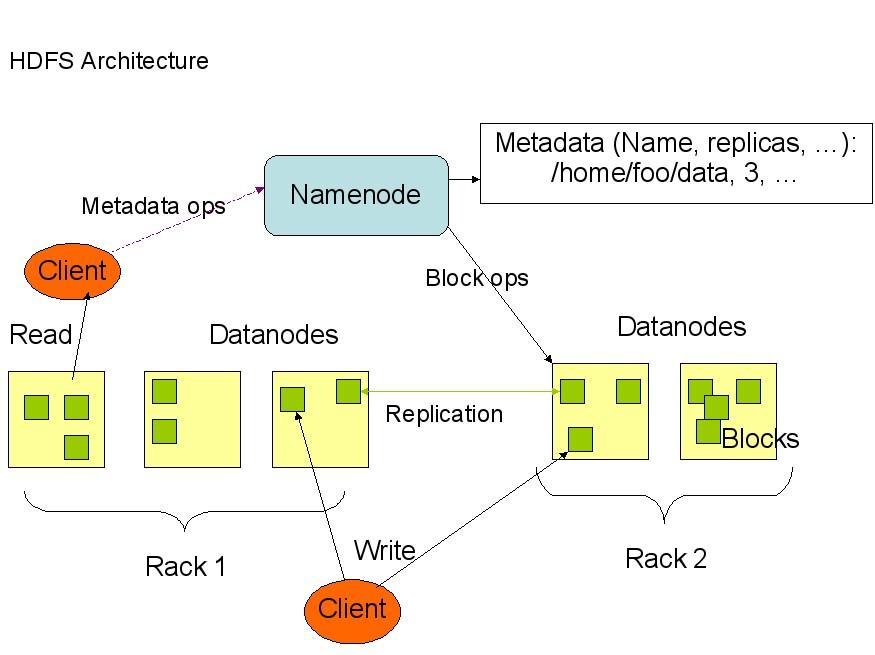
\includegraphics[scale=0.5]{photo/HDFS.jpg}
\caption{HDFS架构}
\end{figure} 


  第二个部分是MapReduce编程模型。为了进行大数据量的计算,通常采用并行计算方法。MapReduce可以简化并行计算。

\section{一些解决方案}
  为了实现大量数据的实时性查询,主要有以下几种方案:
\subsection{RDBMS}
  典型的代表就是Mysql。它的优点有:模式固定,具有ACID性质和复杂的SQL查询处理引擎,能够保证数据的一致性和完整性。但另一方面,他也有许多难以避免的缺点,主要有:在上亿条记录里进行查询效率十分低下,无法进行简单的扩展。


  为了将Mysql满足海量数据查询的需要,就必须进行扩展为关系型数据库集群。当前的思路是随着数据量的增加,使得单点的结构变为主从型的分布,这样就能在从节点进行读操作,缓解了读操作时造成的IO压力。另外,如果数据库中的表数目较多,则可以将不同的表分开存储;如果某一个表太大,则可以把表分为不同的分区同样进行分布式存储。


\tikzstyle{block}=[rectangle,draw,fill=blue!20,text width=5em,
text centered,rounded corners,minimum height=4em]
\tikzstyle{line} = [draw, very thick, color=black!50]

\begin{tikzpicture}[node distance=3cm]
\node [block] (first) {单点db};
\node [block,right of=first] (second) {主从分布};
\node [block,right of=second] (third) {纵向切割};
\node [block,right of=third] (fourth) {横向切割};
\path [line] (first) -- (second);
\path [line] (second) -- (third);
\path [line] (third) -- (fourth);
\end{tikzpicture}

\subsection{Hive}
  Hive是建立在Hadoop上的数据仓库基础构架。它提供了一系列的工具,可以用来进行数据提取转化加载(ETL),这是一种可以存储、查询和分析存储在Hadoop中的大规模数据的机制。Hive定义了简单的类SQL查询语言,称为QL,它允许熟悉SQL的用户查询数据。同时,这个语言也允许熟悉MapReduce开发者的开发自定义的mapper和reducer 来处理内建的mapper和reducer 无法完成的复杂的分析工作。\cite{dataprocess}\cite{webfenxi}介绍了Hive的特点和日志分析的应用。


  下图是hive的架构: 


\begin{figure}[!ht]
\centering
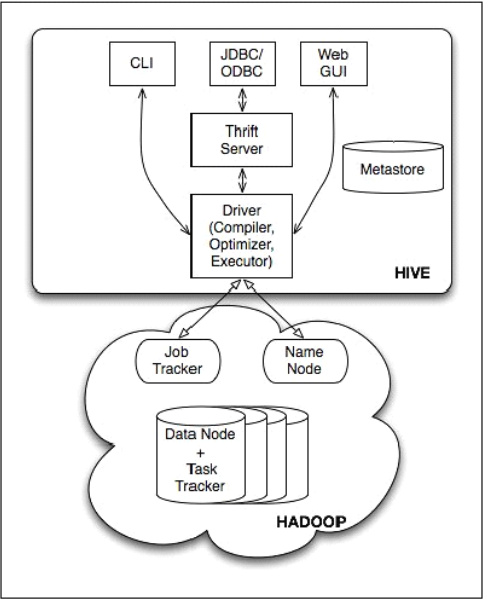
\includegraphics[scale=0.6]{photo/hive.PNG} 
\caption{Hive的架构图}
\end{figure} 


  Hive的用户接口包括CLI,Client和WUI。其中最常用的是CLI,Cli启动的时候,会同时启动一个Hive副本。Client是Hive的客户端,用户连接至HiveServer。在启动Client模式的时候,需要指出HiveServer所在节点,并且在该节点启动HiveServer。WUI是通过浏览器访问Hive。


  Hive将元数据存储在数据库中,如mysql、derby。Hive中的元数据包括表的名字,表的列和分区及其属性,表的属性(是否为外部表等),表的数据所在目录等。


  解释器、编译器、优化器完成HQL查询语句从词法分析、语法分析、编译、优化以及查询计划的生成。


生成的查询计划存储在HDFS中,并在随后有MapReduce调用执行。Hive的数据存储在HDFS中,大部分的查询由MapReduce完成。

\subsection{HBase}
  HBase ,是一个高可靠性、高性能、面向列、可伸缩的分布式存储系统,利用HBase技术可在廉价PC Server上搭建起大规模结构化存储集群。


  HBase是Google Bigtable的开源实现,类似Google Bigtable利用GFS作为其文件存储系统,HBase利用Hadoop HDFS作为其文件存储系统;Google运行MapReduce来处理Bigtable中的海量数据,HBase同样利用Hadoop MapReduce来处理HBase中的海量数据;Google Bigtable利用 Chubby作为协同服务,HBase利用Zookeeper作为对应。


  下图是HBase的架构图: 


\begin{figure}[!ht]
\centering
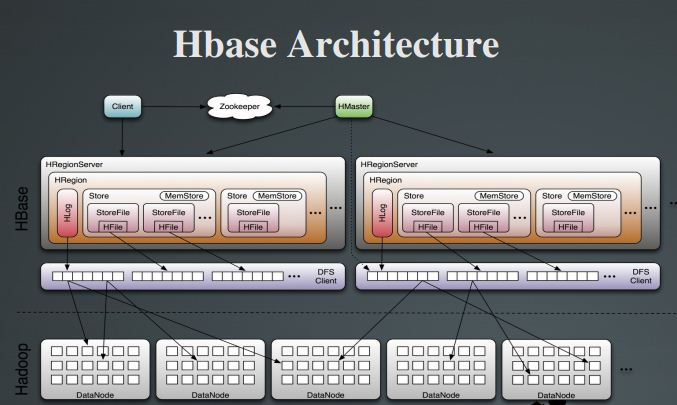
\includegraphics[scale=0.5]{photo/hbase.JPG}
\caption{HBase的架构图}
\end{figure}


  HBase的表由行和列组成,列划分为若干个列族。表中的row key是用来检索记录的主键,访问表中的行可以通过单个row key访问,也可以通过row key的range,还有就是全表扫描。行的一次读写是原子操作。


  Hbase表中的每一列都归属于某个列族,列族是表的chema的一部分(而列不是),必须在使用表之前定义,列名都以列族作为前缀。访问控制、磁盘和内存的使用统计都是在列族层面进行的。下面是一个表的示例:
\clearpage

\begin{figure}[!ht]
\centering
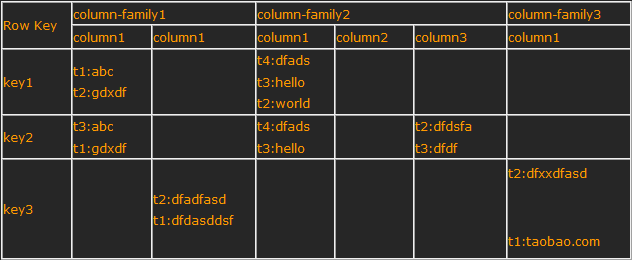
\includegraphics[]{photo/hbaseTable.PNG} 
\caption{HBase的表结构}
\end{figure} 

  从上面的表结构可以看出,Hbase的列不仅可以为空,亦可以动态进行增加,这就相对比较灵活。此外,Hbase的存储是自动分片的,少了人工操作的麻烦。它的缺点是没有一个功能强大的查询引擎,不支持复杂查询。

\subsection{MongoDB}
MongoDB是一个介于关系数据库和非关系数据库之间的产品,是非关系数据库当中功能最丰富,最像关系数据库的。他支持的数据结构非常松散,是类似json的bjson格式,因此可以存储比较复杂的数据类型。Mongo最大的特点是他支持的查询语言非常强大,其语法有点类似于面向对象的查询语言,几乎可以实现类似关系数据库单表查询的绝大部分功能,而且还支持对数据建立索引。\cite{MongoDBGuide}这本书比较详细的介绍了MongoDB的特性。

它的特点是高性能、易部署、易使用,存储数据非常方便。主要功能特性有:
\begin{compactitem}
\item 面向集合存储,易存储对象类型的数据。
\item 模式自由。
\item 支持动态查询。
\item 支持完全索引,包含内部对象。
\item 支持查询。
\item 支持复制和故障恢复。
\item 使用高效的二进制数据存储,包括大型对象(如视频等)。
\item 自动处理碎片,以支持云计算层次的扩展性。
\item 支持RUBY,PYTHON,JAVA,C++,PHP等多种语言。
\item 文件存储格式为BSON(一种JSON的扩展)。
\item 可通过网络访问。
\end{compactitem}

\chapter{研究方法}
  本课题主要目的是为了着重在实时性方面进行主要的研究。所以总的研究采用了横向比较的思路,即在各个不同的解决方案如RDBMS和NOSQL之间进行控制变量的比较。整个比较的过程分为基础性的调研,并在实验的基础上得出结论。而后根据实验的结果进行实时性上的优化。采取各种各样的方法力图将每一个查询处理所用到的延迟时间降到最低,以期满足性能上的要求。


  基础性调研具体来说就是将相同的查询应用到同一数据上进行对比。这里的查询包括常见的简单查询和复杂查询,如连接查询;这里的数据分为小数量级和大数量级;这里的比较内容主要是查询所消耗的时间,即实时性指标;这里的比较是在mysql、hive、hbase和mongoDB之间。

  
  改进的过程具体来说就是充分发挥各个开源产品的优点,能够分布式的进行分布式查询,能够将表结构进行优良设计的进行优良设计,能够修改相关参数的争取把参数调到最优,能够改进实现算法的改进实现算法。以完成查询处理的最佳实践。


\section{Hive和HBase的整合}
  由于非关系型数据库hbase不提供条件查询的接口,但是作为一个面向列簇的NOSQL数据库它又具有自己独特的优点。为了能够较为方便的实现HBase的条件查询,考虑到hive的查询引擎使用的方便性,我们这里利用到了apache Hbase官方网站\footnote{http://wiki.apache.org/hadoop/Hive/HBaseIntegration
}上提供的整合工具hive-hbase-handler.jar实现二者的整合。

\subsection{原理}
图2-1是这种方法的实现原理。


\begin{figure}[!ht]
\centering
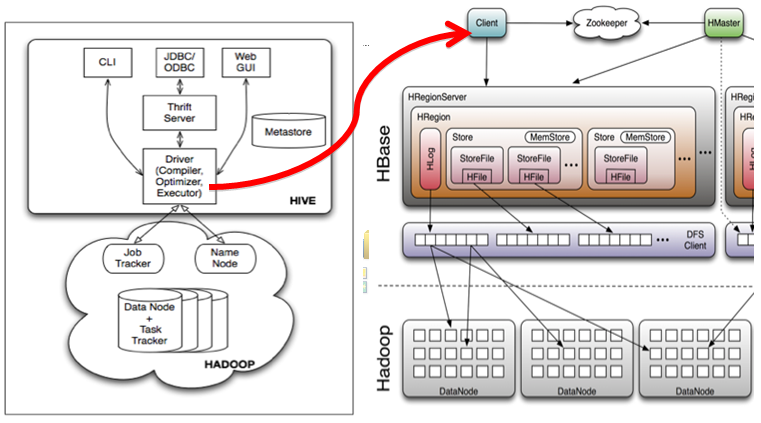
\includegraphics[scale=0.8]{photo/hive-hbase.PNG} 
\caption{Hive和HBase整合的原理}
\end{figure} 


  如图所示,左边的部分是hive的架构图,之前的hive是直接建立在Hadoop集群之上的,也就是说hive作为一个查询引擎驱动直接操作HDFS中存放的数据。而现在可以将Hive作为Hbase的client,这样一来就能够通过hive来实现数据的条件查询,复杂查询等等,另一方面数据还是存在HBase中的。总体的效果就是hive中插入的数据无论在hive还是在hbase中都能看到而且效果一样。同理,在hbase中修改数据后在Hive中查询得到的结果也会随之改变。

\subsection{整合的过程}
\begin{enumerate}
\item 将hbase-0.90.5.jar和zookeeper-3.3.2.jar拷贝到hive/lib下。
注意:如何hive/lib下已经存在这两个文件的其他版本(例如zookeeper-3.3.1.jar),建议删除后使用hbase下的相关版本。


拷贝hbase-site.xml到hive/conf目录下(我在没拷贝时出现过hbase master not running exception,拷贝后就好了)。

拷贝hbase/conf下的hbase-site.xml文件到所有hadoop节点(包括master)的hadoop/conf下。

这一部分就是通过拷贝配置文件使得hive和hbase互相了解对方的版本和具体的配置细节,以便于handler调用。

\item 在\$HIVE\_HOME/conf 目录中修改文件hive-site.xml:

\begin{figure}[!ht]
\centering
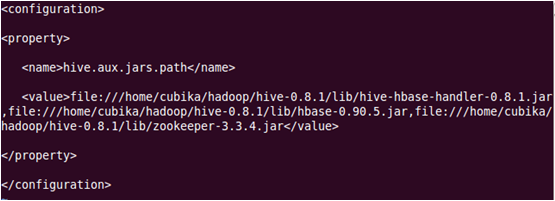
\includegraphics[]{photo/hive-site.PNG} 
\caption{hive-site.xml的设置}
\end{figure} 

如图所示,这个配置文件的意思就是在启动时指定了各个软件的jar包的路径,这样启动后的handler就可以调用相应的jar包。

\item 单节点启动方法:
bin/hive –hiveconf hbase.master=master:60000
集群启动方法:
bin/hive –hiveconf hbase.zookeeper.quorum=slave


\item  创建hbase识别的表:

\begin{lstlisting}[language=SQL]
CREATE TABLE hbase_table_1(key int, value string)  
STORED BY 'org.apache.hadoop.hive.hbase.HBaseStorageHandler'  
WITH SERDEPROPERTIES ("hbase.columns.mapping" = ":key,cf1:val")  
TBLPROPERTIES ("hbase.table.name" = "xyz");
\end{lstlisting}


创建表时需要注意到的两点是:1.存储时用到了HBaseStorageHandler,这个工具的作用就是可以用它来创建新的HBase表格、删除HBase中的表格等等。2.指定时加入映射的关系,即hbase.columns.mapping,将hive表中的某一列映射为hbase的某一列族的某一列,在指定时必须要明确用:key来使某一列称为Hbase的rowkey,另外映射前后表的列数必须相同。

\item 导入数据

\begin{lstlisting}[language=SQL]
hive> CREATE TABLE pokes (foo INT, bar STRING); 
hive> LOAD DATA LOCAL INPATH './examples/files/kv1.txt' OVERWRITE INTO TABLE pokes;
hive> INSERT OVERWRITE TABLE hbase_table_1 SELECT * FROM pokes WHERE foo=86;
\end{lstlisting}

这样就在整合后的表hbase\_table\_1中插入了一条记录foo=86。

\item 分别在hive中和hbase中查看数据

在hive中查看:
\begin{lstlisting}[language=SQL]
hive> select * from  hbase_table_1;
\end{lstlisting}

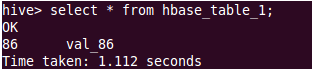
\includegraphics[]{photo/integration-hive.png}

在hbase中查看:
\begin{lstlisting}[language=SQL]
hbase(main):001:0> describe 'xyz'   
hbase(main):002:0> scan 'xyz'
\end{lstlisting}

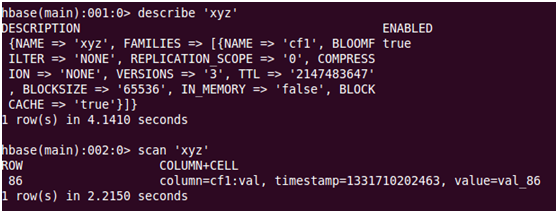
\includegraphics[]{photo/integration-hbase.png}

  从上两幅图中可以看出,无论对于hive中存在的表hbase\_table\_1还是hbase中的表xyz,他们两个已经息息相关,他们两个表中的数据是一样的,而且对任何一个表进行插入操作都会引起两个表的查询结果同时改变,这说明二者已经紧密结合。
\end{enumerate}

\section{数据导入}
在基础性调研之前首先需要做的工作是进行各个表格的创建以及数据的导入。数据的导入方法随着数据库的不同而不同,但基本上大同小异。由于导入时数据量可以很大,导入的时间消耗其实也可以作为一项实时性的性能指标。

\subsection{将数据导入到hive}
  这里导入的文件格式是csv -- 逗号分隔型取值格式(英文全称为Comma Separated Values,简称CSV)。它是一种纯文本格式,用来存储数据。在CSV中,数据的字段由逗号分开,程序通过读取文件重新创建正确的字段。hive中对于不同的格式有不同的导入方法,下面介绍hive导入csv格式文本文件的具体步骤。

\begin{enumerate}

\item 从https://github.com/ogrodnek/csv-serde 下载hive导入csv的serde包,在hive里将这个包的路径添加进来: add jar /home/cloud/csv-serde-1.1.2.jar。有了这个jar包才能进行csv格式文本的导入工作。

\item 创建表bicc
这是一个电信的表格,每一项是一宗通话的各个具体的信息。建表语句为:

\begin{lstlisting}[language=SQL]
CREATE TABLE bicc
(
  START_TIME_S             string,
  START_TIME_NS            string,
  END_TIME_S               string,
  END_TIME_NS              string,
  CDR_INDEX                string,
  SOURCE_IP                string,
  DESTINATION_IP           string,
  CIC                      string,
  OPC                      string,
  DPC                      string,
  RELEASE_REASON           string,
  CALLING_NUMBER           string,
  CALLED_NUMBER            string,
  ORIGINAL_CALLED_NUMBER   string,
  TRANSFER_NUMBER          string,
  LOCATION_NUMBER          string,
  RESPONSE_TIME            string,
  ACM_TIME                 string,
  ANM_TIME                 string,
  REL_TIME                 string,
  CALL_DURATION            string,
  DURATION                 string,
  CODEC_MODIFY_FLAG        string,
  CODEC_MODIFY_RESULT      string,
  CODEC_NEGOTIATION_FLAG   string,
  CODEC_NEGOTIATION_RESULT string,
  CODEC_TYPE               string,
  CALL_TYPE                string,
  IS_EXT_PLATFORM          string,
  CALL_HOLD                string,
  CALL_FORWARD             string,
  CALL_WAITING             string,
  CONFRENCE_CALL           string
)
row format serde 'com.bizo.hive.serde.csv.CSVSerde'
stored as textfile;
\end{lstlisting}

这里的row format其实是使用了刚刚添加的jar包CSVSerde,目的就是告诉hive如何判断每一个域,具体来说就是以逗号作为每个域的分隔符,换行作为每个行的分隔符。

\item 插入数据:
插入了100个记录,插入的源是文件bicc\_100.csv
\begin{lstlisting}
bin/hadoop fs -put /home/cloud/data/bicc_100.csv /user/hive/warehouse/bicc
\end{lstlisting}
因为这里hive数据仓库在HDFS中的路径就是/user/hive/warehouse,将文件直接放到这个目录下的bicc目录里其实也是相当于在这个表中插入了数据。另外用hive提供的LOAD DATA INPATH语法插入数据也可以。


  同理可以新建两个大数据量的表格:yuyin(380万个记录)和duanxin(940万个记录)。这两个表的结构是一样的,同样是:“用户号码|漫游类型|区号呼叫发生地|呼叫日期|呼叫时间|长途类型|方向类型|通话时长|位置小区代码|蜂窝号基站代码|”,建表的语句和上面类似,在这里就不在赘述了。
\end{enumerate}

\subsection{将数据导入到hive/hbase中}
经过整合之后,hive/hbase的所有操作和hive是完全一样的,唯一的不同就是需要首先启动hbase服务。因为只有开启了hbase服务后handler才能打开hbase中的表。下面是向整合后的表插入数据的各个具体步骤。
\begin{enumerate}

\item 创建hive和hbase整合后的表 SRC\_TBD\_BICC\_CDR,这个表对应了上述的表bicc。建表语句是:

\begin{lstlisting}[language=SQL]
create table SRC_TBD_BICC_CDR
(
  START_TIME_S             string,
  START_TIME_NS            string,
  END_TIME_S               string,
  END_TIME_NS              string,
  CDR_INDEX                string,
  SOURCE_IP                string,
  DESTINATION_IP           string,
  CIC                      string,
  OPC                      string,
  DPC                      string,
  RELEASE_REASON           string,
  CALLING_NUMBER           string,
  CALLED_NUMBER            string,
  ORIGINAL_CALLED_NUMBER   string,
  TRANSFER_NUMBER          string,
  LOCATION_NUMBER          string,
  RESPONSE_TIME            string,
  ACM_TIME                 string,
  ANM_TIME                 string,
  REL_TIME                 string,
  CALL_DURATION            string,
  DURATION                 string,
  CODEC_MODIFY_FLAG        string,
  CODEC_MODIFY_RESULT      string,
  CODEC_NEGOTIATION_FLAG   string,
  CODEC_NEGOTIATION_RESULT string,
  CODEC_TYPE               string,
  CALL_TYPE                string,
  IS_EXT_PLATFORM          string,
  CALL_HOLD                string,
  CALL_FORWARD             string,
  CALL_WAITING             string,
  CONFRENCE_CALL           string
)
STORED BY 'org.apache.hadoop.hive.hbase.HBaseStorageHandler'  
WITH SERDEPROPERTIES 
("hbase.columns.mapping"=" START_TIME:START_TIME_S,:key,END_TIME:END_TIME_S,END_TIME:END_TIME_NS,INDEX:CDR_INDEX,IP:SOURCE_IP,IP:DESTINATION_IP,C:CIC,C:OPC,C:DPC,REASON:RELEASE_REASON,NUMBER:CALLING_NUMBER,NUMBER:CALLED_NUMBER,NUMBER:ORIGINAL_CALLED_NUMBER,NUMBER:TRANSFER_NUMBER,NUMBER:LOCATION_NUMBER,TIME:RESPONSE_TIME,TIME:ACM_TIME,TIME:ANM_TIME,TIME:REL_TIME,DURATION:CALL_DURATION,DURATION:DURATION,CODEC:CODEC_MODIFY_FLAG,CODEC:CODEC_MODIFY_RESULT,CODEC:CODEC_NEGOTIATION_FLAG,CODEC:CODEC_NEGOTIATION_RESULT,TYPE:CODEC_TYPE,TYPE:CALL_TYPE,PLATFORM:IS_EXT_PLATFORM,CALL:CALL_HOLD,CALL:CALL_FORWARD,CALL:CALL_WAITING,CALL:CONFRENCE_CALL")
TBLPROPERTIES ("hbase.table.name" = "BICC_CDR");
\end{lstlisting}

同理这里指定了各个列的对应关系。
\item 插入数据

\begin{lstlisting}[language=SQL]
INSERT OVERWRITE TABLE src_tbd_bicc_cdr SELECT a.* FROM bicc a;
\end{lstlisting}
将数据从表bicc中拷贝到表src\_tbd\_bicc\_cdr中。

\begin{figure}[!ht]
\centering
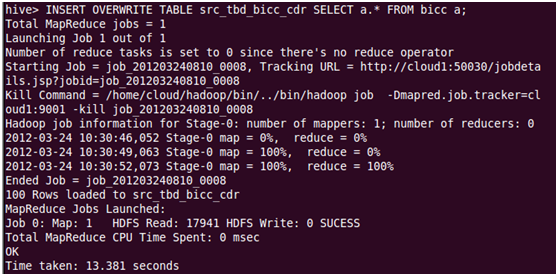
\includegraphics[]{photo/insert-bicc-hive.png}
\caption{src\_tbd\_bicc\_cdr表的插入时间}
\end{figure} 

\item 查看插入后的结果:
\clearpage
\begin{figure}[!ht]
\centering
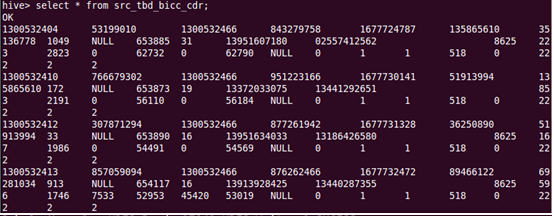
\includegraphics[]{photo/select-bicc-hive.png}
\caption{查看hive表}
\end{figure} 

再查看hbase表:
\begin{figure}[!ht]
\centering
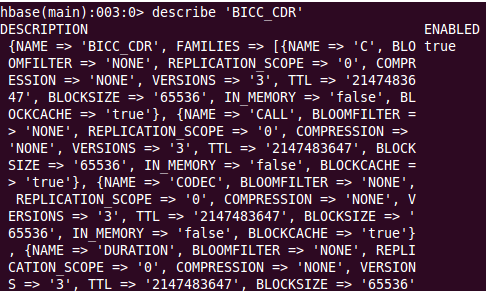
\includegraphics[]{photo/scan-bicc-hbase.png}
\caption{查看hbase表}
\end{figure} 

\end{enumerate}

同理可以对应于上述的大表yuyin和duanxin建立相应的表hbase\_yuyin和hbase\_duanxin。以下是它们插入数据所用的时间:
\clearpage

\begin{figure}[!ht]
\centering
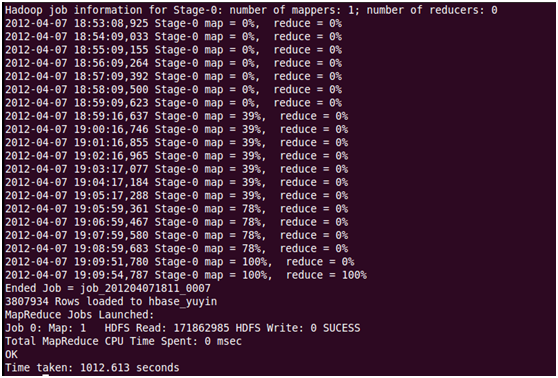
\includegraphics[scale=0.8]{photo/insert-yuyin-hbase.png} 
\caption{yuyin表的插入时间}
\end{figure} 

\begin{figure}[!ht]
\centering
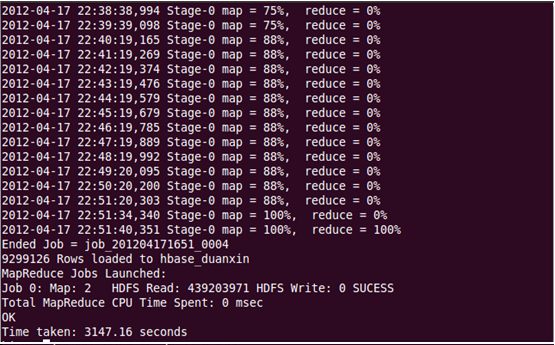
\includegraphics[scale=0.8]{photo/insert-duanxin-hbase.png}
\caption{duanxin表的插入时间}
\end{figure} 

\subsection{导入数据到mongoDB}
对于mongoDB来说,有其自带的导入工具mongoimport,这个工具的使用方法可以在官方的文档上找到\footnote{http://www.mongodb.org/display/DOCS/Import+Export+Tools\#ImportExportTools-mongoimport}。由于mongoDB面向文档,所以不用事先建立一个表,而是直接可以从文本文件中导入,需要制定相应的域就可以了。
这里给出我使用的例子:
\begin{lstlisting}
./mongoimport -d "mydb" -c "bicc" -f "start_time_s,start_time_ns,end_time_t,end_time_ns,cdr_index,source_ip,destination_ip,cic,opc,dpc,release_reason,calling_number,called_number,original_called_number,transfer_number,location_number,response_time,acm_time,anm_time,rel_time,call_duration,codec_modify_flag,codec_modify_result,codec_negotiation_flag,codec_negotiation_result,codec_type,call_type,is_ext_platform,call_hold,call_forward,call_waiting,conference_call" --type csv --file /mnt/hgfs/home/data/bicc_100.csv
\end{lstlisting}
数据量小时导入很快,当导入数据量很大时就需要消耗一定的时间。如下图所示:
\begin{figure}[!ht]
\centering
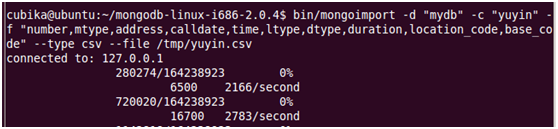
\includegraphics[]{photo/mongoimport.png} 
\caption{yuyin表的插入时间}
\end{figure} 
从图中可以看出整个导入过程花了3000秒左右。

\subsection{导入数据到mysql中}
导入时首先建立表,再进行插入。建表语句为:
\begin{lstlisting}[language=SQL]
create table duanxin
(
key int,
number string,
mtype int,
address string,
calldate string,
time string,
ltype int,
dtype int,
duration int,
location_code string,
base_code string
)
row format delimited 
fields terminated by '|'
stored as textfile;
\end{lstlisting}

插入语句为:
\begin{lstlisting}
LOAD DATA LOCAL INPATH '/home/cloud/data/ 清单数据/ 数据部分/duanxin2.txt' OVERWRITE INTO TABLE duanxin;
\end{lstlisting}
\chapter{查询实验结果}
  根据上一章提到的研究思路,在导入了数据之后就可以在其之上进行对比性的查询实验。查询时尽量采用一些典型的测试用例,场景分为大小两种数量级的简单和复杂的情形。总共是四种情况,下面先来看小数量级的简单查询情形。

\section{简单查询}
\subsection{小数量级}

  这个实验使用了已经建好的表格bicc,它只有100个记录,简单查询时采用了两个具体的测试用例。其中第一个用例是:

\begin{lstlisting}[language=SQL]
select cic from bicc where cic>100 and cic<500;
\end{lstlisting}

然后我们来看一下这个查询分别在hive、hbase、mysqL和mongoDB下所得到的实验结果:
\begin{description}

\item
\begin{figure}[h]
\begin{minipage}[t]{0.45\linewidth}
\centering
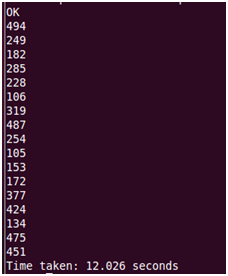
\includegraphics[width=0.8\textwidth]{photo/xjh1.png}
\caption{hive表的查询时间}
\end{minipage}
\hfill
\begin{minipage}[t]{0.45\linewidth}
\centering
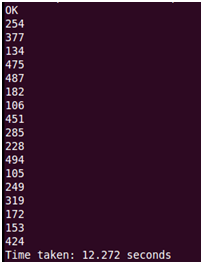
\includegraphics[width=0.8\textwidth]{photo/xjh2.png}
\caption{hive/hbase表的查询时间}
\end{minipage}
\end{figure}

\clearpage

\item
\begin{figure}[!ht]
\centering
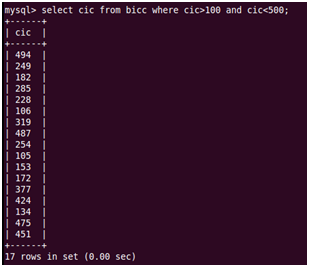
\includegraphics[scale=0.9]{photo/xjm1.png} 
\caption{mysql表的查询时间}
\end{figure} 

\item
\begin{figure}[!ht]
\centering
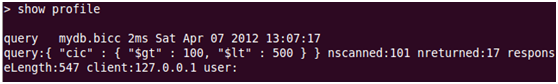
\includegraphics[]{photo/xjm2.png} 
\caption{mongoDB表的查询时间}
\end{figure} 
\end{description}

从这个实验得到的结果可以看出,hive和hive/hbase的结果是一个数量级,均在12s左右,而mysql和mongoDB所耗费的时间在一个数量级,差不多是3ms以下。他们之间的差别还是很大的。


第二个用到的测试用例是:
\begin{lstlisting}[language=SQL]
 select cic from bicc where cic<100 order by cic desc;
\end{lstlisting}

即从表bicc中挑出cic列值小于100的记录并且递减排序。这个查询最后得到的结果如图3-5到图3-8所示:
\begin{description}

\item
\begin{figure}[h]
\begin{minipage}[t]{0.45\linewidth}
\centering
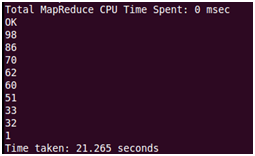
\includegraphics[width=0.8\textwidth]{photo/xjh3.png}
\caption{hive表的查询时间}
\end{minipage}
\hfill
\begin{minipage}[t]{0.45\linewidth}
\centering
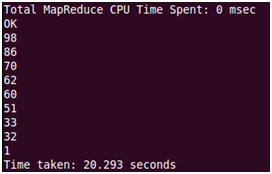
\includegraphics[width=0.8\textwidth]{photo/xjh4.png}
\caption{hive/hbase表的查询时间}
\end{minipage}
\end{figure}

\item
\begin{figure}[!ht]
\centering
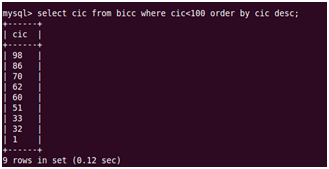
\includegraphics[]{photo/xjm3.png} 
\caption{mysql表的查询时间}
\end{figure} 

\item
\begin{figure}[!ht]
\centering
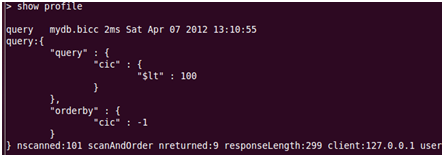
\includegraphics[]{photo/xjm4.png} 
\caption{mongoDB表的查询时间}
\end{figure} 

\end{description}
从第二个测试用例中得到的结果可以看出和由第一个测试用例得出的结果是一致的。

\subsection{大数量级}

  在小型数据级上做的实验放到大数据集上又会有不一样的结论。在原来基础上将实验用到的数据量加到很大,具体来说这里用到了已经建好的表yuyin,它拥有380万个记录,以及规模更大的表duanxin,它拥有940万个记录。同样也是采取两个测试用例加以互相验证,其中使用的第一个测试用例为:
\begin{lstlisting}[language=SQL]
select number from yuyin where ltype=4 and dtype=4;
\end{lstlisting}

这个语句很简单,实验的结果可以从图3-9到图3-12看出:
\clearpage
\begin{description}

\item
\begin{figure}[h]
\begin{minipage}[t]{0.4\linewidth}
\centering
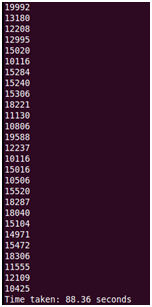
\includegraphics[width=0.7\textwidth,height=7cm]{photo/djh1.png}
\caption{hive表的查询时间}
\end{minipage}
\hfill
\begin{minipage}[t]{0.4\linewidth}
\centering
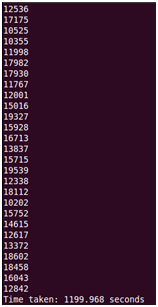
\includegraphics[width=0.7\textwidth,height=7cm]{photo/djh2.png}
\caption{hive/hbase表的查询时间}
\end{minipage}
\end{figure}

\item
\begin{figure}[!ht]
\centering
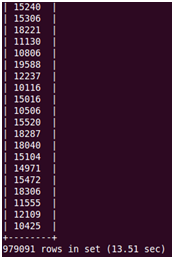
\includegraphics[]{photo/djm1.png} 
\caption{mysql表的查询时间}
\end{figure} 

\item
\begin{figure}[!ht]
\centering
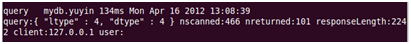
\includegraphics[scale=1.2]{photo/djm2.png} 
\caption{mongoDB表的查询时间}
\end{figure} 

\end{description}

从上面几个图中可以清晰的看到,hive查询用了88s,而hive/hbase查询足足用了1200s,mysql用了13s,mongoDB由于只查询头20条结果,因此时间不足一秒。可以看出hive相对来说较之前有所提升,而hive/hbase则相对下降,所花费的时间也达到了很难容忍的地步。为了对这个结果加以验证,我们又使用了第二个测试用例:
\begin{lstlisting}[language=SQL]
select distinct number from yuyin where duration<60 order by number desc;
\end{lstlisting}

实验的结果可以从图3-13到图3-16看出:
\begin{description}

\item
\begin{figure}[h]
\begin{minipage}[t]{0.4\linewidth}
\centering
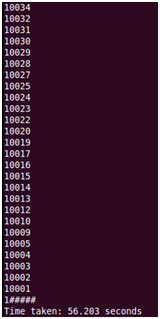
\includegraphics[width=0.7\textwidth,height=7cm]{photo/djh3.png}
\caption{hive表的查询时间}
\end{minipage}
\hfill
\begin{minipage}[t]{0.4\linewidth}
\centering
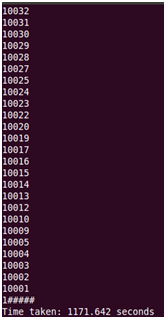
\includegraphics[width=0.7\textwidth,height=7cm]{photo/djh4.png}
\caption{hive/hbase表的查询时间}
\end{minipage}
\end{figure}

\item
\begin{figure}[!ht]
\centering
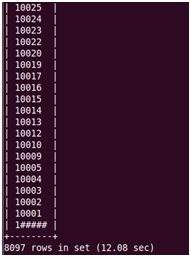
\includegraphics[]{photo/djm3.png} 
\caption{mysql表的查询时间}
\end{figure} 

\item
\begin{figure}[!ht]
\centering
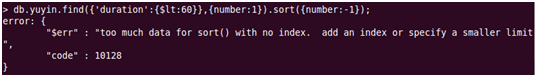
\includegraphics[]{photo/djm4.png} 
\caption{mongoDB表的查询时间}
\end{figure} 

\end{description}
从上面结果可以看出,hive用了56s,hive/hbase用了1171s,mysql用了12s,整体来说还是和第一个测试用例得到的结果是一致的。即时间hive/hbase>hive>mysql。

380万行的数据查询已经说明了一些问题,如果继续地增加数据量会有什么变化呢?接下来测试一下940万行的表duanxin,这里采用的测试用例为:
\begin{lstlisting}[language=SQL]
select distinct address from duanxin where mtype=0 and ltype=0;
\end{lstlisting}

实验的结果可以从图3-17到图3-19看出:
\begin{description}

\item
\begin{figure}[!ht]
\centering
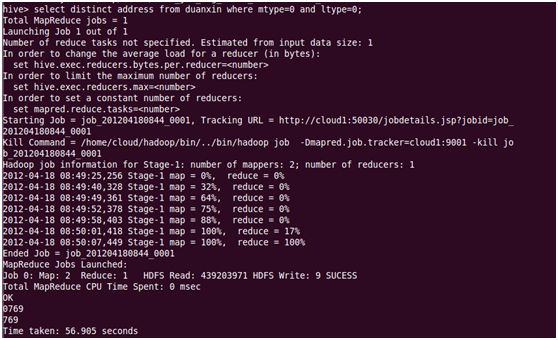
\includegraphics[scale=0.8]{photo/djh5.png}
\caption{hive表的查询时间}
\end{figure} 

\item
\begin{figure}[!ht]
\centering
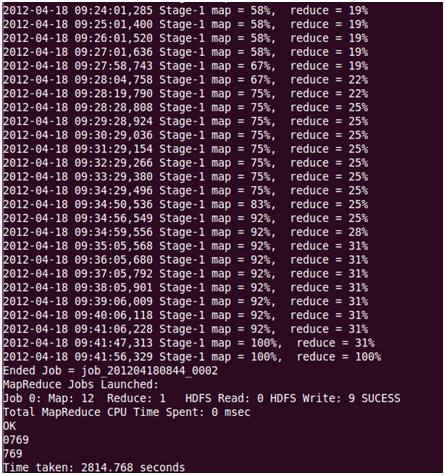
\includegraphics[scale=0.7]{photo/djh6.png}
\caption{hive/hbase表的查询时间}
\end{figure} 

\item
\begin{figure}[!ht]
\centering
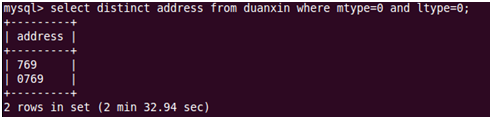
\includegraphics[]{photo/djm5.png} 
\caption{mysql表的查询时间}
\end{figure} 

\end{description}
从上三个图中可以看出,hive查询用了56秒,hive/hbase用了2814秒,mysql用了153秒。hive相对于mysql来说性能逐渐上升,到这时已经超出mysql达到最快,而hive/hbase这种方法的性能更加恶化,将近用了46分钟的时间,而hive花了不到一分钟。可想差别有多大。

\section{复杂查询}
复杂查询有很多种,比如嵌套查询等等。但最为典型的就是两个表之间的连接查询了。因此接下来的所有复杂查询都是指连接查询。而连接查询又分为很多种,如内连接,外连接等等。我们这里只考虑等值连接的情况。

\subsection{小数量级}
 由于表bicc和bssap表的结构相似,我们首先将这两个表进行等值连接。选取start\_time\_s这一项作为比较项。SQL语句为:
\begin{lstlisting}[language=SQL]
select distinct a.start_time_s join bssap b on a.start_time_s=b.start_time_s;
\end{lstlisting}

实验的结果可以从图3-20到图3-22看出:
\begin{description}

\item
\begin{figure}[h]
\begin{minipage}[t]{0.45\linewidth}
\centering
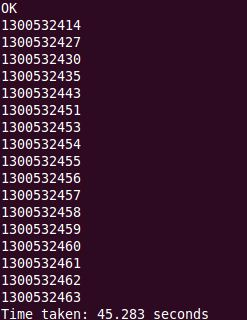
\includegraphics[width=0.8\textwidth,height=7cm]{photo/xfh1.png} 
\caption{hive表的查询时间}
\end{minipage}
\hfill
\begin{minipage}[t]{0.45\linewidth}
\centering
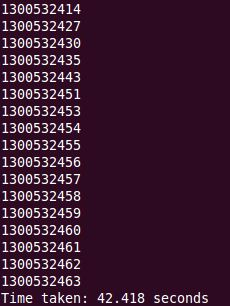
\includegraphics[width=0.8\textwidth,height=7cm]{photo/xfh2.png} 
\caption{hive/hbase表的查询时间}
\end{minipage}
\end{figure}

\item
\begin{figure}[!ht]
\centering
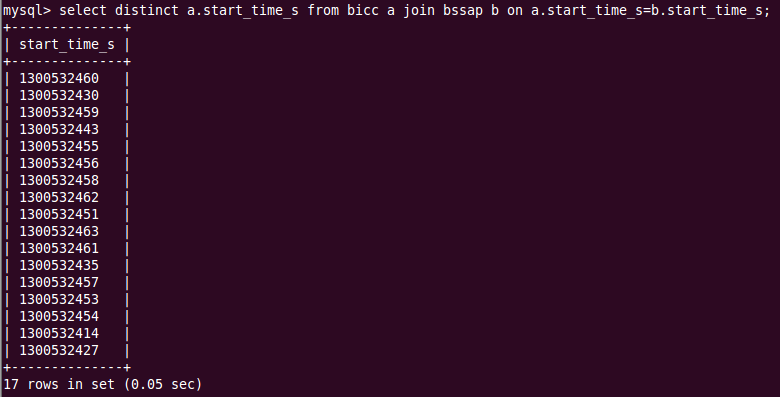
\includegraphics[width=0.8\linewidth]{photo/xfm1.png} 
\caption{mysql表的查询时间}
\end{figure} 

\end{description}
由于这两个表都非常小,join时花费的时间还是很少的。但仍然可以看出mysql远远快于hive和hive/hbase。

\subsection{大数量级}

将已经建好的表yuyin和表duanxin进行join等值连接:
\begin{lstlisting}[language=SQL]
select count(distinct a.address) from yuyin a join duanxin b on a.number=b.number;
\end{lstlisting}

由于表的规模太大,所以采用了让程序在服务器后台运行的方法。为了准确计算时间,我编写了shell脚本调用各个程序并计算调用程序前后的时间差,转换后的结果为秒。图3-23和3-24显示了hive和hive/hbase的脚本。

\begin{figure}[!ht]
\centering
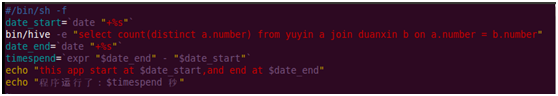
\includegraphics[]{photo/jb1.png} 
\caption{hive执行脚本}
\end{figure} 

\begin{figure}[!ht]
\centering
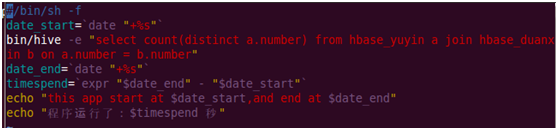
\includegraphics[]{photo/jb3.png} 
\caption{hive/hbase执行脚本}
\end{figure} 

后台执行脚本时输入:
\begin{lstlisting}[language=sh]
nohup ./h1.sh > h1out.txt 2>&1 &;
\end{lstlisting}
这样执行的结果就重定向到h1out.txt文本文件中。

mysql执行时也采取同样的办法。但是mysql第一次运行时出现“MySQL client ran out of memory”的错误。经过查阅资料,发现mysql分别使用mysql\_store\_result和mysql\_use\_result这两种方法存储结果集。mysql\_store\_result方法是把结果集全部存储在内存中,而mysql\_use\_result不把结果集存在客户端内存中,而是按需去mysql服务器取。由于这个连接查询结果集太大,如果用mysql\_store\_result的方法是放不下内存的,所以需要改用第二个方案。在执行时加入--quick选项。除此之外,由于结果太大,磁盘空间很可能不足,可以采用mysql提供的格式化结果的选项,使用grep命令只将带有时间的一行输出。

本次使用了count命令使得程序的输出没有受到磁盘空间的困扰,完整的mysql执行脚本为:
\begin{figure}[!ht]
\centering
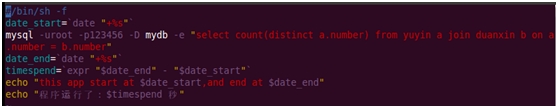
\includegraphics[]{photo/jb2.png} 
\caption{mysql执行脚本}
\end{figure} 



最后,实验的结果可以从图3-26到图3-28看出:
\begin{description}

\item
\begin{figure}[!ht]
\centering
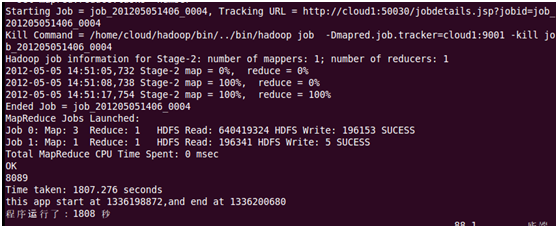
\includegraphics[]{photo/dfh1.png} 
\caption{hive表的查询时间}
\end{figure} 

\clearpage
\item
\begin{figure}[!ht]
\centering
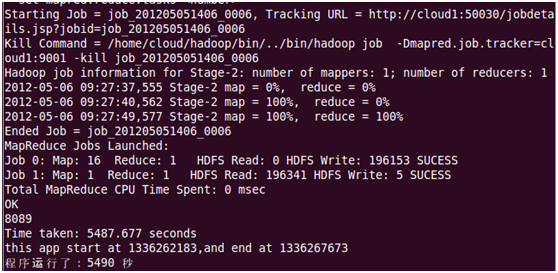
\includegraphics[]{photo/dfh2.png} 
\caption{hive/hbase表的查询时间}
\end{figure} 

\item
\begin{figure}[!ht]
\centering
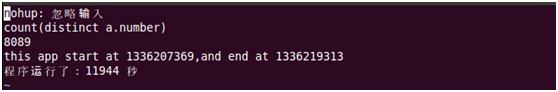
\includegraphics[]{photo/dfm1.png} 
\caption{mysql表的查询时间}
\end{figure} 

\end{description}
可以看出hive用了1808秒,hive/hbase用了5490秒,mysql用了11944秒。mysql执行的时间明显高于其他。

\section{总结}

\begin{table}[!h]
\arrayrulewidth=1pt
\centering
{\Large
\begin{tabular}{|c|c|c|c|}\hline
\rowcolor{gray!50} & hive & hive/hbase & mysql \\\hline
\rowcolor{green!60}简单查询(100行) & 12s-20s & 12s-20s & 0ms-100ms \\\hline
\rowcolor{green!20} 简单查询(380万行) & 88s & 1200s  & 14s \\\hline
\rowcolor{green!60} 简单查询(940万行) & 57s & 2814s & 153s \\\hline
\rowcolor{green!20} 复杂查询(小数量级) & 45s & 42s & 5ms \\\hline
\rowcolor{green!60} 复杂查询(大数量级) & 1808s & 5490s & 11944s \\\hline
\end{tabular}
}
\caption{实验数据汇总}
\end{table}


\chapter{查询优化}
在实际的操作中,不同的查询需要采取不同的实现方法。有时候查询语句往往一个小的改动都会造成完全不一样的时间消耗,这一点在大型数据上的表现尤其的明显。所以,在实际的执行过程中要特别注重查询的效率问题,结合数据库理论和具体的环境进行不同的优化工作。优化的方法有很多种,根据我的查找和思考,以及\cite{youhua},\cite{youhuayanjiu}的介绍,这里仅仅介绍我个人认为比较重要的几个方面。

\section{使用索引}
我们知道,索引是数据库中十分重要的一个概念,如果使用的合理适当,能够极大幅度的提高效率。从某种意义上来说,索引可以理解为一种特殊的目录。索引中保存着表中存储的索引列,并且记录了索引列在数据库表中的物理存储位置,实现了表中数据的逻辑索引。在没有索引时,查询需要进行全表的扫描,将每一条的记录取出并和查询条件一一对比,这无疑会消耗大量的时间并且造成许多磁盘IO。有了索引之后,就可以直接在索引中找到符合条件的索引值,将相应的指针返回就能够找到需要的记录。因此,有了索引可以避免全表扫描,也就可以大大减少时间。这和通过目录查找相应的内容的道理是一样的,要比一页一页的翻肯定来得快。


需要注意的是,索引也是一个单独的物理结构,建立索引需要花费空间和时间的代价,它也是要占用物理空间的。更加重要的是,一旦表中的记录发生了变化如增加删除和修改等等,索引本身也要相应的调整,因此要适当考虑创建和维护索引的代价,想好究竟哪些字段需要建立索引,不能一味建立索引。


事实上,索引的建立是有一定的原则的。如对于查询中很少涉及到的列或者重复值比较多的列不需要建立索引;对于按范围查询的列最好建立索引;表中若有主键或者外键一定要建立索引;而对于一些特殊的数据类型,如文本字段TXT,图像类型字段IMAGE等等,由于长度不定,很难建立索引。


一般数据库中的索引分为唯一索引、主键索引和聚集索引。唯一索引就是不允许任何两行有相同索引值的索引;主键索引是为主键所准备,它唯一表示了这一行;聚集索引是使得表的索引顺序和物理顺序一样,一个表只能包含一个聚集索引。


根据索引的特点一般来说,下面的几种情况下建立索引最为有效:
\begin{compactitem}
\item
在经常进行连接的字段上建立索引。
\item
在频繁进行groupby 和orderby,即排序或者分组操作的列上建立索引。
\item
在条件表达式中经常用到的不同值较多的列上建立索引。
\item
如果待排序的列有多个,可以在这些列上建立复合索引。
\end{compactitem}

接下来我们通过一个例子来验证索引的作用:

\begin{lstlisting}[language=SQL]
// 查询语句 
select calldate,time from duanxin where calldate>100600 and time>110000 group by calldate;

// 建立索引 
create index date_time on duanxin(calldate(6),time(6));

// 使用索引 
select calldate,time from duanxin force index(date_time) where calldate>100600 and time>110000 group by calldate;
\end{lstlisting}

下面是建立索引前后的对比:
\begin{figure}[h]
\begin{minipage}[t]{0.4\linewidth}
\centering
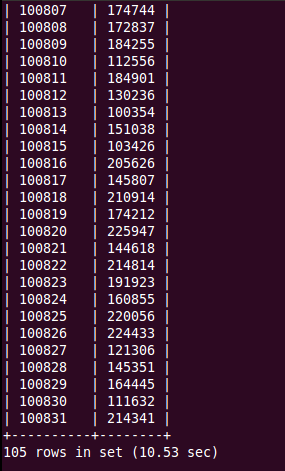
\includegraphics[width=0.7\textwidth,height=7cm]{photo/index1.png}
\caption{建立索引前}
\end{minipage}
\hfill
\begin{minipage}[t]{0.4\linewidth}
\centering
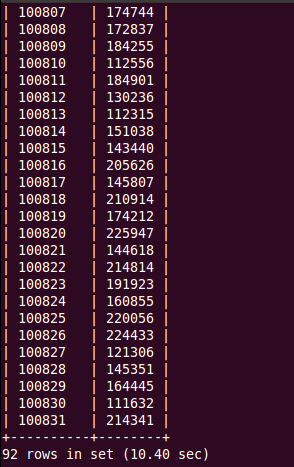
\includegraphics[width=0.7\textwidth,height=7cm]{photo/index2.png}
\caption{建立索引后}
\end{minipage}
\end{figure}

\section{参数优化}
在实际应用中,设定参数可以调优查询代码的执行效率。这里仅仅讨论hive的参数优化问题。

\subsection{如何设定参数}
首先说明的是,对于一般的参数,大概有三种设定方式:
\begin{compactitem}
\item 配置文件
\item 命令行参数
\item 参数声明
\end{compactitem}
其中配置文件就是conf文件夹下的文件,可以是默认的,也可以是用户自己定义的配置文件。配置文件的设定对本机启动的所有Hive进程都有效。而命令行参数就是在启动hive时,在命令行添加 -hiveconf param=value来设定。参数声明就是在HQL中使用SET关键字设定,如set mapred.reduce.tasks=100.后两种设定的作用域是Session级的。

\subsection{列裁剪(Column Pruning)}
在读数据的时候,只读取查询中需要的列,而忽略其他列。例如表T 包含 5 个列 (a,b,c,d,e),当实现查询

\begin{lstlisting}[language=SQL]
SELECT a,b FROM T WHERE e < 10;
\end{lstlisting}

这样列 c,d 将会被忽略,只会读取a, b, e 列。这个选项默认为真:hive.optimize.cp = true

\subsection{分区裁剪(Partition Pruning)}
在查询时减少不必要的分区。例如:

\begin{lstlisting}[language=SQL]
SELECT * FROM (SELECT c1, COUNT(1)
  FROM T GROUP BY c1) subq
  WHERE subq.prtn = 100;

SELECT * FROM T1 JOIN
  (SELECT * FROM T2) subq ON (T1.c1=subq.c2)
  WHERE subq.prtn = 100;
\end{lstlisting}

会在子查询中就考虑 subq.prtn = 100 条件,从而减少读入的分区数目。
此选项默认为真:hive.optimize.pruner=true。

\subsection{Join和MapJoin}
首先应该将条目少的表/子查询放在 Join 操作符的左边。因为join操作符左边的表的内容会被加载进内存。另外,在多个表进行join时,如果join的key值是相同的,那么将会合并成一个MapReduce任务,如果不同,则任务数目和join操作的数目相同。


join的方法有reduce端的join和map端的join之分,其中reduce端的join的工作就是把两个表都生成key-value对,在reduce端进行笛卡尔积;mapjoin的原理就是把小表全部读入内存中,在map阶段直接拿另外一个表的数据和内存中表数据做匹配。换句话说,只将大表生成key-value对,由于小表非常的小,足以在内存中放下并且可以进行全表的扫描,因此在map端就可以将小表中的值全部取出并匹配,避免了笛卡尔乘积。\cite{mapjoin}.


下面是一个使用mapjoin的例子:

\begin{lstlisting}[language=SQL]
SELECT /*+ MAPJOIN(x) */ x.key, x.value, y.valueFROM src1 x LEFT OUTER JOIN src y ON (x.key = y.key);
\end{lstlisting}

再次强调mapjoin仅仅适用于一个小表和一个大表join的场景。因此这里的表x一定是小表。如果太大会出现内存不足的错误。

\subsection{groupby}
hive.map.aggr = true 是否在 Map 端进行聚合,默认为 True 
hive.groupby.mapaggr.checkinterval = 100000 在 Map 端进行聚合操作的条目数目 
hive.groupby.skewindata = false 有数据倾斜的时候进行负载均衡 

\subsection{合并小文件}
文件数目过多,会给 HDFS 带来压力,并且会影响处理效率,可以通过合并 Map 和 Reduce 的结果文件来消除这样的影响:
\begin{compactitem}
\item hive.merge.mapfiles = true 是否和并 Map 输出文件,默认为 True 
\item hive.merge.mapredfiles = false 是否合并 Reduce 输出文件,默认为 False 
\item hive.merge.size.per.task = 256*1000*1000 合并文件的大小 
\end{compactitem}

\section{对join查询算法的研究}
参考文献\cite{join}比较详细的介绍了各种join的算法。标准的join算法可以通过MapReduce的一个Job实现。在map阶段通过提取需要join的key,生成一个标签tag,再加上value形成一个(key,value)对。这个标签标志了这条记录来源于哪一个表。接下来将他们进行排序与合并。在reduce阶段,对于每一个key,根据标签来把每一个value值划分为左右两个缓冲区,该记录来源于两个表中的哪个表就放到哪个缓冲区里。然后进行笛卡尔积就可以得到结果。伪代码可以表示为:
\begin{lstlisting}
Map(K:null,V:a record from a split of either R or L)
  join_key ← extract the join column from V
  tagged_record ← add a tag of either R or L to V
  emit(join_key,tagged_record)

Reduce(K′: a join key,LISTV′: r ecords from R and L with join key K′)
create buffers BR and BL for R and L, respectively
for each record t in LISTV′do
append t to one of the buffers according to its tag
for each pair of records (r, l) in BR×BL do
emit(null , newrecord(r,l))
\end{lstlisting}

这个算法的实现在hadoop自带的例子datajoin里面有。代码如下:
\begin{lstlisting}[language=Java]
//SampleDataJoinMapper.java
public class SampleDataJoinMapper extends DataJoinMapperBase {


  protected Text generateInputTag(String inputFile) {
    // tag the row with input file name (data source)
    return new Text(inputFile);
  }

  protected Text generateGroupKey(TaggedMapOutput aRecord) {
    // first column in the input tab separated files becomes the key (to perform the JOIN)
    String line = ((Text) aRecord.getData()).toString();
    String groupKey = "";
    String[] tokens = line.split("\\t", 2);
    groupKey = tokens[0];
    return new Text(groupKey);
  }

  protected TaggedMapOutput generateTaggedMapOutput(Object value) {
    TaggedMapOutput retv = new SampleTaggedMapOutput((Text) value);
    retv.setTag(new Text(this.inputTag));
    return retv;
  }
}

//SampleDataJoinReducer.java
public class SampleDataJoinReducer extends DataJoinReducerBase {
  protected TaggedMapOutput combine(Object[] tags, Object[] values) {
    // eliminate rows which didnot match in one of the two tables (for INNER JOIN)
    if (tags.length < 2)
       return null;  
    String joinedStr = ""; 
    for (int i=0; i<tags.length; i++) {
      if (i > 0)
         joinedStr += "\t";
      // strip first column as it is the key on which we joined
      String line = ((Text) (((TaggedMapOutput) values[i]).getData())).toString();
      String[] tokens = line.split("\\t", 2);
      joinedStr += tokens[1];
    }
    TaggedMapOutput retv = new SampleTaggedMapOutput(new Text(joinedStr));
    retv.setTag((Text) tags[0]); 
    return retv;
  }
}

//SampleDataOutput.java
public class SampleTaggedMapOutput extends TaggedMapOutput {

  private Text data;

  public SampleTaggedMapOutput() {
    this.data = new Text("");
  }

  public SampleTaggedMapOutput(Text data) {
    this.data = data;
  }

  public Writable getData() {
    return data;
  }

  public void write(DataOutput out) throws IOException {
    this.tag.write(out);
    this.data.write(out);
  }

  public void readFields(DataInput in) throws IOException {
    this.tag.readFields(in);
    this.data.readFields(in);
  }
}
\end{lstlisting}

这个算法的问题在于对两个表都需要进行缓冲,数据量很大时表不一定能完全放到内存缓冲区里。针对这个问题有许多种改进方法。第一个改进就是将标签放到value里,形成value\_tag的方式,这样便于对两个表分别进行排序。第二个改进就是无论在map阶段还是reduce阶段都对join\_key生成hash值,这样便于查找。最后的改进方法包括只将相对较小的表进行缓冲,然后再生成join的结果。
\begin{lstlisting}
Map(K: null , V: a record from a split of either R or L)
joinkey ← extract the join column from V
tagged record ← add a tag of either R or L to V
compositekey ← (joinkey, tag)
emit(compositekey, taggedrecord)
Partition(K: input key)
hashcode ← hashfunc(K.joinkey)
return hashcode mod # reducers

Reduce(K′: a composite key with the join key and the tag 
LISTV′: records for K′, first from R, then L)
create a buffer BR for R
for each R record r in LISTV′do
store r in BR
for each L record l in LISTV′do
for each record r in BR do
emit(null , newrecord(r, l))
\end{lstlisting}

还有一个改进可以是首先进行预处理操作,针对join\_key先进行分块,这样在以后的join操作之前都避免了相同操作,直接的进行join就行了。
\chapter{HBase客户端编程}
我们知道,HBase有很多访问接口,其中,HBase Shell是HBase的命令行工具,它最简单,适合HBase管理使用;Thrift Gateway,它利用Thrift序列化技术,支持C++,PHP,Python等多种语言,适合其他异构系统在线访问HBase表数据;REST Gateway,支持REST 风格的Http API访问HBase, 解除了语言限制
;还有就是我们这一章用到的Native Java API访问方式,他是最常规和高效的访问方式,适合Hadoop MapReduce Job并行批处理HBase表数据。用户可以通过编写Java程序来对HBase中存在的表进行新建删除、对记录进行插入删除以及查询等等。编程时用到的api可以从官方网站\footnote{http://hbase.apache.org/apidocs/index.html}上查到非常详细的介绍。下面介绍几个客户端编程用到的重要概念:

\section{客户端编程的重要概念}

\subsection{HBaseConfiguration}
HBaseConfiguration是每一个hbase client都会使用到的对象,它代表的是HBase配置信息。
默认的构造方式会尝试从hbase-default.xml和hbase-site.xml中读取配置。如果classpath没有这两个文件,就需要你自己设置配置。
\begin{lstlisting}[language=Java]
Configuration HBASE_CONFIG = new Configuration();
HBASE_CONFIG.set(“hbase.zookeeper.quorum”, “zkServer”);
HBASE_CONFIG.set(“hbase.zookeeper.property.clientPort”, “2181″);
HBaseConfiguration cfg = new HBaseConfiguration(HBASE_CONFIG);
\end{lstlisting}

\subsection{HBaseAdmin}
HBaseAdmin负责表的META信息处理。创建和删除表都是通过HBaseAdmin来操作的。其中创建表时使用HBaseAdmin提供的createTable这个方法,并可以通过addFamily方法增加列族。删除表之前要disableTable,然后再进行deleteTable操作。下面代码是创建表和删除表的示例:

\begin{lstlisting}[language=Java]
//创建表
HBaseAdmin hAdmin = new HBaseAdmin(hbaseConfig);
HTableDescriptor t = new HTableDescriptor(tableName);
t.addFamily(new HColumnDescriptor(“f1″));
t.addFamily(new HColumnDescriptor(“f2″));
t.addFamily(new HColumnDescriptor(“f3″));
t.addFamily(new HColumnDescriptor(“f4″));
hAdmin.createTable(t);

//删除表
HBaseAdmin hAdmin = new HBaseAdmin(hbaseConfig);
if (hAdmin.tableExists(tableName)) {
       hAdmin.disableTable(tableName);
       hAdmin.deleteTable(tableName);
}
\end{lstlisting}

\subsection{Put和Get/Scan}
Put方法用来向HTable中插入数据,可以通过以下两种方法插入单个数据或者批量插入:
\begin{lstlisting}[language=Java]
public void put(final Put put) throws IOException
public void put(final List<Put> puts) throws IOException
\end{lstlisting}

get方法可以实现通过rowkey在table中查询某一行的数据,getScanner方法可以通过指定一段rowkey范围来查询。

\begin{lstlisting}[language=Java]
public Result get(final Get get)
public ResultScanner getScanner(final Scan scan)
\end{lstlisting}

get/scan可以通过addFamily/addColumn方法指定family或者column;通过setFilter来过滤信息;Scan可以通过setStartRow和setStopRow来指定开始和结束的行。结果是Result对象,可以通过result的getRow,getValue等方法获取详细信息。下面是两个例子:

\begin{lstlisting}[language=Java]
//通过 row 获取 data
       public static void getbyrow(HTable table, String row) throws IOException { 
                 Get get=new Get(row.getBytes()); 
                 Result r = table.get(get); 
                 print(r); 
       }   
 } 

//返回所有data
public static void getAllData(HTable table) throws IOException { 
          Scan s = new Scan(); 
          ResultScanner rs = table.getScanner(s); 
           for (Result r : rs) { 
                   print(r); 
           } 
} 
\end{lstlisting}

\subsection{Filters}
Hbase中的Filter是用来进行过滤查询信息的,HBase本身提供了多种多样的Filter。
比较类型的Filter包括RowFilter,它可以根据rowkey来进行过滤,FamilyFilter可以根据列族的比较来过滤,类似的还有QualifierFilter和ValueFilter。专用的Filter包括SingleColumnValueFilter,它可以根据值来决定是否返回该行,PrefixFilter可以根据行首信息来过滤,PageFilter指定一页中可以返回多少行,KeyOnlyFilter只考虑key值而忽略value值。此外还有许许多多的Filter。一次可以使用多个Filter,可以把不同的Filter放到一个FilterList里面。

详细信息可以查看\cite{HBaseGuide}这一本书中更加详细的介绍。

\section{应用实例}
对应前面的条件查询实验,这里我通过使用SingleColumnValueFilter来实现 select * from yuyin where ltype=4 and dtype=4 的查询。

\subsection{代码}

\begin{lstlisting}[language=Java]
import java.io.IOException;
import java.util.ArrayList;
import java.util.List;

import org.apache.hadoop.conf.Configuration;
import org.apache.hadoop.hbase.HBaseConfiguration;
import org.apache.hadoop.hbase.KeyValue;
import org.apache.hadoop.hbase.client.Get;
import org.apache.hadoop.hbase.client.HTable;
import org.apache.hadoop.hbase.client.Result;
import org.apache.hadoop.hbase.client.ResultScanner;
import org.apache.hadoop.hbase.client.Scan;
import org.apache.hadoop.hbase.filter.FilterList;
import org.apache.hadoop.hbase.filter.SingleColumnValueFilter;
import org.apache.hadoop.hbase.filter.CompareFilter.CompareOp;
import org.apache.hadoop.hbase.util.Bytes;

import org.apache.hadoop.hbase.HConstants;

public class ValueFilter {

    private static Configuration conf = null;

    /** 
     * 初始化配置 
     */
    static {
        conf = HBaseConfiguration.create();

//设置timeout 为120s
conf.setLong(HConstants.HBASE_REGIONSERVER_LEASE_PERIOD_KEY, 120000);
    } 
     
 public static void selectByFilter(String tablename,List<String> arr) throws IOException{   
        HTable table=new HTable(conf,tablename);   
        FilterList filterList = new FilterList();
        Scan s1 = new Scan();
        for(String v:arr){ // 各个条件之间是“与”的关系   
            String [] s=v.split(",");
            filterList.addFilter(new SingleColumnValueFilter(Bytes.toBytes(s[0]),Bytes.toBytes(s[1]),
                       CompareOp.EQUAL,Bytes.toBytes(s[2]) )
            );
            // 添加下面这一行后,则只返回指定的cell,同一行中的其他cell不返回   
         s1.addColumn(Bytes.toBytes(s[0]), Bytes.toBytes(s[1]));   
        }
        s1.setFilter(filterList);
        ResultScanner ResultScannerFilterList = table.getScanner(s1);
        for(Result rr=ResultScannerFilterList.next();rr!=null;rr=ResultScannerFilterList.next()){
            for(KeyValue kv:rr.list()){
                System.out.println("row : "+new String(kv.getRow()));
                System.out.println("column : "+new String(kv.getFamily()));
                System.out.println("value : "+new String(kv.getValue()));
            }
        }
    }

    public static void  main (String [] agrs) throws IOException {
        long start= System.currentTimeMillis();
        List<String> arr=new ArrayList<String>();
        // select * from yuyin where ltype=4 and dtype=4;
        arr.add("type,ltype,4");
		 arr.add(“type,dtype,4”);
        ValueFilter.selectByFilter("yuyin",arr);
        long end= System.currentTimeMillis();
        System.out.println("time spend: "+(end-start)/1000+"s");
}
}
\end{lstlisting}
首先将查询条件放到一个List里面,将List中的字符串通过逗号分开生成字符串数组s,s[0]是hbase中的column family,s[1]是column family下对应的column,s[2]是相应的value。通过scan对象调用setFilter方法进行过滤,通过table.getScanner方法得到类型为ResultScanner的结果。逐个遍历ResultScanner的内容就可以打印出相应的信息。

\subsection{编译并打包}
\begin{lstlisting}[language=Java]
// 编译 
javac -cp $HBaseClassPath:$JAVA_HOME/lib/*.jar ValueFilter.java

// 打包 
jar -cvf ValueFilter.jar ValueFilter.class
\end{lstlisting}

编译时指定各种jar包,包括hadoop core的包,hbase 版本的包,hbase lib文件夹下的所有jar包等等。通过指定这些jar包的路径作为classpath,就能成功的生成class文件,即java的字节码。编译之后的打包工作是为了hadoop调用。

\subsection{执行}
\begin{lstlisting}[language=Java]
~/hadoop/bin/hadoop jar ValueFilter.jar ValueFilter
\end{lstlisting}

执行的结果为:
\begin{figure}[!ht]
\centering
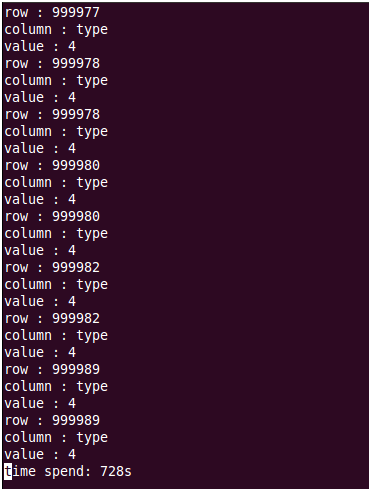
\includegraphics[scale=0.5]{photo/bcjg.png} 
\caption{mongoDB表的查询时间}
\end{figure} 

可以看出,经过了编译、打包、执行等一系列工作,最终的结果是能够准确的返回符合条件的记录集。
%%%%%%%%%%%%%%%%%%% 参考文献 %%%%%%%%%%%%%%%%
\songti\zihao{5}
\bibliographystyle{IEEEtran}
\bibliography{IEEEabrv,data/reference}
\addcontentsline{toc}{chapter}{参考文献}

%%%%%%%%%%%%%%%%%%%%% 致谢 %%%%%%%%%%%%%%%%%%
\chapter*{致\qquad 谢}
\songti\zihao{-4}

  本次毕设的完成我得到了很多人的帮助。首先要感谢的是我的指导老师侯宾,从最初的开题到中间的每一周的开展我都得到了侯宾老师非常耐心的指导,不仅使我对自己的毕设有了更深入的了解,而且对于未来工作如何开展、对于整体情况的把握都有非常重要的帮助。另外还要感谢卓海艺学长对我的细心指导和帮助,正是他和我共同探讨了毕设的设计,并且在我遇到问题时给了我正确的纠正,还有一直以来对我的支持。此外还要感谢我的室友闭美春指导我论文格式的排版工作。

  本次毕设所做的工作相对来说比较基础,由于个人能力和时间等问题,特别是在优化这方面还有不少可以改进的地方,希望在未来能够加以改善。
\addcontentsline{toc}{chapter}{致谢}

%%%%%%%%%%%%%%%%%%%%% 译文 %%%%%%%%%%%%%%%%%%
\pdfbookmark[0]{译文}{translation}
\pagestyle{empty}

\chapter*{外\quad 文\quad 译\quad 文}

\begin{center}
{\heiti\zihao{3}Distributed Semantic Web Data Management in HBase and MySQL Cluster \\
\textsl{By Craig Franke, Samuel Morin, Artem Chebotko, John Abraham, and Pearl Brazier}

\heiti 在HBase和MySQL集群中的分布式语义WEB的数据管理
}
\end{center}

\zihao{-4}

\section*{摘要}
在互联网上的各种各样的计算型资源和数据资源正通过机器解释的语义描述方式得到增强,以便于更好的搜索、发现和集成。这个由相互关联的元数据构成的语义Web,它的容量能潜在地增加着整个互联网的规模。语义Web数据的高效管理,通过W3C的资源描述框架进行表述,对于支持新型的数据密集型语义的应用来说是非常关键的。在本次工作中,我们研究并比较了两种基于新兴的云计算技术和传统的关系型数据集群技术的分布式RDF数据管理方法。特别的,我们为HBase和MySQL集群设计了分布式RDF数据存储和查询方案,并且在the Third Provenance Challenge和Lehigh大学的机器集群上通过使用基准数据集和查询对这些方法进行了实证比较。我们的研究结果揭示了有趣的查询评估模式,这表明了我们的算法是拥有前途的,而且暗示了对于可扩展的语义Web数据管理来说云计算有很大的潜力。


\section*{综述}
  万维网联盟(W3C)推荐并标准化了一系列的规则则、语言、框架和连接各种各样的元数据到下一代互联网的最佳实践,那就是语义Web。W3C的元数据获取语言包括资源描述框架(RDF),RDFa(属性),RDFs(模式),Web本体语言(OWL)。政府、学术界和产业界积极的拥抱这些技术来捕获和共享语义Web的元数据。举几个例子,oeGOV正在为电子市场制定和发布OWL本体,美国人口普查数据正以RDF的形式发布,生物信息学家以RDF的方式维持通用蛋白质资源,地球科学家出版全球范围的地里的RDF数据库GeoNames,美国最大的电子产品零售商百思买以RDF的方式发布它所有的产品目录,美国最大的社交网络提供商Facebook使用RDFa在它的网页中嵌入元数据。服务计算社区通过使用了例如OWL-S、WSDL-S、SWSO等词汇的语义注释,增强了现有的语义Web服务。


  RDF数据模型是一个直接的,标识的图形,他也可以被序列化为一组三元关系。本论文中的例子包括10个描述了使用LUBM词汇的三元组,如图1所示。每个三元组由一个主体,谓词和对象组成,并且定义了一个主体和对象之间的关系。图中<>和“”分别表示资源标识符和一些个数据类型。例如,前三个三元组的资源标识符C是一个学生,拥有名字Craig并且是IEEE的成员。这个示例数据集可以使用SPARQL语言来查询,它是一个RDF的标准查询语言。SPARQL使用三元模型和图形模型来匹配RDF数据。例如从包含?X< type ><UndergraduateStudent>模式的LUBM中的Q14查询返回所有本科生标志并赋给X变量。关于SPARQL特性和语义更多的细节可以在W3C的SPARQL规范中发现。

  随着语义Web的快速发展和作为元数据的主要语言的RDF的广泛应用,RDF数据有效的管理将会对于支持新型的在不同领域的语义应用来说是至关重要的。许多研究人员建议使用关系型数据库存储和查询大型的RDF数据集。这种被称作关系型RDF数据库或者关系型RDF商店的系统现在正被频繁地应用在产品中。最近,在云计算中广泛使用的分布式技术如Hadoop何Hbase等,正用来开发分布式的和可扩展的RDF数据管理。据我们所知,这项工作提供了在Hbase和MysQL集群中使用我们的设计和算法解决方案来进行存储和查询RDF数据的关键性能的比较。

  本篇论文的主要贡献有:(i)用来在HBase中存储RDF数据的新型数据库结构设计(ii)为由我们设计的模式在HBase中进行SPARQL三元组和基本图形的模式匹配提供了有效的算法(iii)高效的SPARQL和SQL之间转换的算法,它能使MySQL集群上进行的SQL查询变得平滑(iv)HBase和MySQL集群上存储和查询语义Web数据的高效和可扩展性的富有经验性的比较。我们的工作展示了在查询评估中有趣的模式,这表明了我们的算法是有希望的,并且暗示了云计算对于可扩展的语义Web的数据管理来说有很大的潜力。

  本篇论文的组织如下:在第二章介绍了相关的工作,第三章和第四章介绍了我们对于HBase和MySQL集群上进行分布式RDF数据的存储和查询的设计和算法,第五章介绍了这两种方法在the Third Provenance Challenge 和Lehigh 大学进行的基准数据集的性能测试报告。最后我们在第六章进行了总结。


\section*{相关工作}
  除了作为google的Bigtable开源实现的HBase,还有很多在Apache基金会下的项目,他们将焦点地方在分布式的计算,这些项目包括Hadoop,Cassandra,Hive,Pig和CouchDB。Hadoop实现了MapReduce软件架构和分布式文件系统。Cassandra将一个完全分布式的设计和面向列的存储融合起来,并且将MapReduce作为支持的特性之一。Hive在Hadoop之上处理数据仓库并且提供了他自己的查询语言HQL。Pig面向于使用它的高层的Pig拉丁语言来书写数据分析程序,这些程序最终被转化为MapReduce工作,以此完成分析大型的数据集。CouchDB是一个分布式的、面向文档的非关系型数据库,它支持JavaScript编写的增量性的MapReduce查询。在学术界和工业界的其他项目,包括Cheetah, Hadoop++, G-Store和HadoopDB都有类似的思路。

 
  接下来简要讨论一下关于分布式RDF数据管理的一些相关工作。参考文献3和6里呈现了评估SPARQL的基本图形模式的技术。参考文献7和8分别提出了在以MapReduce系统中分析型查询处理和RDF图形分布式推理的有效方法。参考文献9和10研究了在点对点的环境下RDF查询处理,11和12报告了分布式RDF源之间联合查询的调解技术。13介绍了在文本索引中HBase的用处。在参考文献14中虽然S声明了spider系统使用了HBase来处理RDF查询处理和扩展的HBase,但是并没有详细的报告。最后,我们之前的工作展示了在HBase中RDF数据管理的最初发现。这篇论文提出了更新更有效的HBase表结构设计,更高效的SPARQL三元组和基本图形模式匹配和算法和对于分布式关系型RDF数据库富有经验的比较。我们的实验比较结果呈现出对于一些查询的数个数量级的提高,以及可扩展性的重大改进。这篇论文和我们之前的论文是关于HBase中语义Web数据管理最先发表的研究成果。我们对于HBase和MySQL集群的RDF数据管理技术的比较也是独一无二的。 

\section*{在Hbase中的分布式RDF数据存储和查询}
  Hbase将数据存储在表中,并且数据可以表述为非常稀疏的多维的排序的映射,这和传统的关系型数据库里的关系非常不同。一个Hbase里的表存储了根据rowkey排序的数据行。每一行有一个唯一的rowkey和任意数量的列,这样在两个不同行的列就不用一模一样。一个列的完整的名称包括一个列族和一个列修饰符,这里的列族是在表建立时就指定的,列族的数量是不会变的,但是列修饰符却可以动态的增加和删除。一个给定行的一列,我们称之为表单元格,能存储一对时间戳值,时间戳在单元格里是惟一的,并且值可以重复。表中的行在Hbase集群不同的机器上可以成为分布式的,并且能进行两个基本的操作:1.表的扫描 2.根据一个给定的rowkey或者列、时间戳等等来检索表格的数据。考虑到对于大数量级来说表格扫描访问路径是非常低效的,以rowkey来检索是最有效的方法。

  
  表格稀疏的特性使得它们称为RDF数据非常富有吸引力的存储选择。RDF图表通常也是很稀松的:不同的资源用不同的属性来注释,并且一些注解可能由于推理的缘故不会显示的指出。为了支持在Hbase表中有效的检索RDF数据,应该考虑到SPARQL构造的基本查询,比如三元模式等等。数据库最起码应该支持RDF三元组的主体、谓词、对象的值的检索。


  我们建议使用两个表的数据库模式来存储RDF三元组,正如图2所示。sp表存储了三元组的主体作为rowkey,三元组的谓词作为列名字,三元组的对象作为单元格的值。op表存储三元组的对象作为rowkey,三元组的谓词作为列名字,三元组的主体作为单元格的值。表2显示了使用我们RDF三元组样例来存储这些表的二维的图形化展示。在这幅图里,s和o代表了rowkey而不是列;类型,名字,属于什么组是列修饰符,这些修饰符属于共同的列族p;{}代表了省略了时间戳的单元格值的集合。更加确切的说,行的这种表结构可以用JavaScript 对象符号来表示为:
\begin{lstlisting}
//the first row of Tsp
<C>:{
  p:{
	type: {t1: <Student> },
	name: {t2: "Carig" },
	memberof:{t3: <IEEE>}
 }
}
//the first row of Top
<Student>:{
 p: {
	type:{ t4:<C>,t5:<S>}
	}
}
\end{lstlisting}

RDF数据建议的模式要求数据本身被存储两次以便用来保证系统的健壮性。表Tsp和Top分别可以根据一致的主体或对象来有效的检索三元组信息。而基于一个谓词的值的检索,由于他需要一个表的全表扫描,因而可能不会非常有效。为了解决这个问题,我们可以创建表Tps或Tpo,将谓词放在rowkey的位置上,而将主体或对象作为列。然而,这样的解决方法只能提供轻微的改善,因为本体的谓词数量通常是比较固定的且相对很小的,这暗示了新的表只能包含大量行的一小部分,而对于任何单一行的检索仍然是代价昂贵的。

为了使Hbase能够评估SPARQL查询,我们设计了三个函数来处理三元组模式和基本图表模式。

我们的第一个函数叫做matchTP-T,是一个通用的函数,它既不依赖于我们的存储模式也不依赖于Hbase。matchTP-T将一个三元模式tp和一个三元组t作为输入,如果他们匹配则返回true,否则返回false。它的伪代码在4中呈现。

算法1中的函数matchTP-DB是用来根据我们的两个表的存储模式来匹配HBase数据库DB中的一个三元组模式tp。这个函数的输出是一个多重集合B,它包含了数据库中所有匹配的三元组。这个算法处理三个不相关的例子。首先,如果tp的主体模式不是一个变量,这个函数从Tsp表中检索出结果。如果tp.pp不是变量,只有拥有了列修饰符tp.pp的列的值从行中检索出来。否则,所有的列都将被检索。由于tp.op可能是也可能不是一个变量,matchTP-T被用在所有的三元组上以除去不匹配的组。在这个过滤之后,B中的组被返回。第二,如果tp的对象模式不是一个变量,这个函数使用相似的方法从表Top中检索出数据。最后,当tp.sp和tp.op都是变量时,其中的一个表必须扫描来检索出所有的行。如果tp.pp不是一个变量,不匹配的列将被舍弃,否则,所有列中的值都将被使用。

  我们最后一个函数matchBGP-DB在算法2中给出轮廓。它将包含了一系列三元组tp1,tp2...的SPARQL基本的图表模式bgp和HBase数据库进行比较,并且返回一个由匹配的三元组组成的图表集合B。这个算法首先使用两个准则来排序bgp中的三元组:(1)为了减少迭代的次数首先应将产出结果小的三元模式放在首位,(2)为了避免不必要的笛卡尔积应将那些有共同变量的三元组优先考虑。作为一个例子,考虑下面的查询和它的排序版本。原来查询中的顺序并不符合所需的条件:tp1在数据集里产生了大量的所有大学里的学生的结果集;tp2和tp1没有公告变量,并且在tp1和tp2之间必须计算耗费内存的笛卡儿积;被记录的查询既能节省内存又能节省网络传输时间:对于三元组tp3,它不仅仅因为有最小结果集它被放在第一位,而且笛卡尔积也被移除了。

  接下来,这个算法使用matchTP-DB算法来评估bgp里的排好序的第一个三元组。如果B中的结果为空,这个算法就不再评估它的子三元组而返回一个空结果集。否则,matchBGP-DB函数就会迭代地计算三元组或者公共变量或者没有公共变量时计算笛卡尔积。每个join连接就像关系型数据库中的连接策略。公共变量首先被B集合中绑定的替换,并使用matchTP-DB函数评估TP集合中的三元组tp'。如果tp'生成了非空的结果,B'中的三元组就将B中相应的三元组串联在一起。

\section*{在Mysql集群中分布式RDF数据存储和查询}
关系型RDF数据库使用几种数据模式产生的方法,包括schema-oblivious,schema-aware等等。这些方法标志了不同的数据库关系,比如属性,类,类的主体和客体及集群化的数据库表等等。在这项工作里,我们使用schema-oblivious方法作用到单个表T(s,p,o)上,这里的列s,p,o相应的存储了三元组的主体,谓词,对象。

  我们选择这一个模式是由于三种原因。首先,它可以支持无模式的修改本体演化。Hbase建议的模式也是非常灵活的,因为只有列的修饰符才会动态的变化而且是在行级上进行变化的。第二,关系型RDF数据库中涉及到的大部分表都可以看作是表水平分区的结果。然而,分区的工作已经被Mysql集群自动的进行了。最后,这个模式允许无损存储,并且很容易实现,特别是它大大的简化了SPARQL到SQL的转换工作,这个工作需要查询存储的RDF数据。

  为了在Mysql集群的数据库架构上执行SPARQL查询,我们提出了一个基本图表模式的SPARQL到SQL的查询转换算法。该算法是以我们以前的工作15为基础,但是它又进行了优化,以生成平坦的SQL查询。平坦的查询会移除一系列在基本图表模式上重新排序的三元组,因为关系型的查询优化器足以自动地选出一个好的连接查询执行序列。

\section*{性能研究}
这一章讨论了在HBase和Mysql集群上进行分布式存储和查询RDF数据的不同方法的经验性比较。
A.实验前提
硬件。我们的实验使用9个有着标准硬件的商业机器。每个机器有3GHz 64bit的奔腾四核处理器,2GB DDR2-533RAM,80GB 7200转串行ATA硬件驱动。机器通过网络连接到一个戴尔巨型以太网交换机,该交换机上安装了64位的Debian Linux和Oracle JDK6。
HBase和Mysql集群。使用了带有更改内核库的Hadoop0.20.2,还有HBase0.90.为了稳定性我们对默认的配置做了细微的更改,包括设置每个数据块复制两次,增加HBase最大堆大小到1.2GB。同时使用了基于快速入门指南配置上更改的Mysql集群7.1.9a,将NDB数据节点使用的内存增加。
我们的实现。我们的算法使用Java语言来实现,并且实验通过使用Bash脚本来自动地和可重复地执行Java类文件和存储的结果。
查询性能评估。Hbase和Mysql集群在PC3和LUBM数据集上的查询性能和可扩展性结果在图4上报告。PC3基准测试送三个不同复杂性的查询:Q1是最简单的查询只用了一个三元组。Q2有三个三元模式,Q3是最复杂的,包括6个模式。所有三个查询里基本的图表模式返回一个小量结果。Hbase和Mysql集群都显示出非常有效的响应时间,而前者稍微的快一点。在第六天,Hbase之前保持的持平的时间也有了轻微的上升,这意味着图有一个小的斜坡(数据集的大小增加了近10倍,而响应时间只有大约2~4倍的增加),类似的行为也在LUBM查询中观察到。

\newpage
\section*{外文译文原文}

\begin{figure}[!ht]
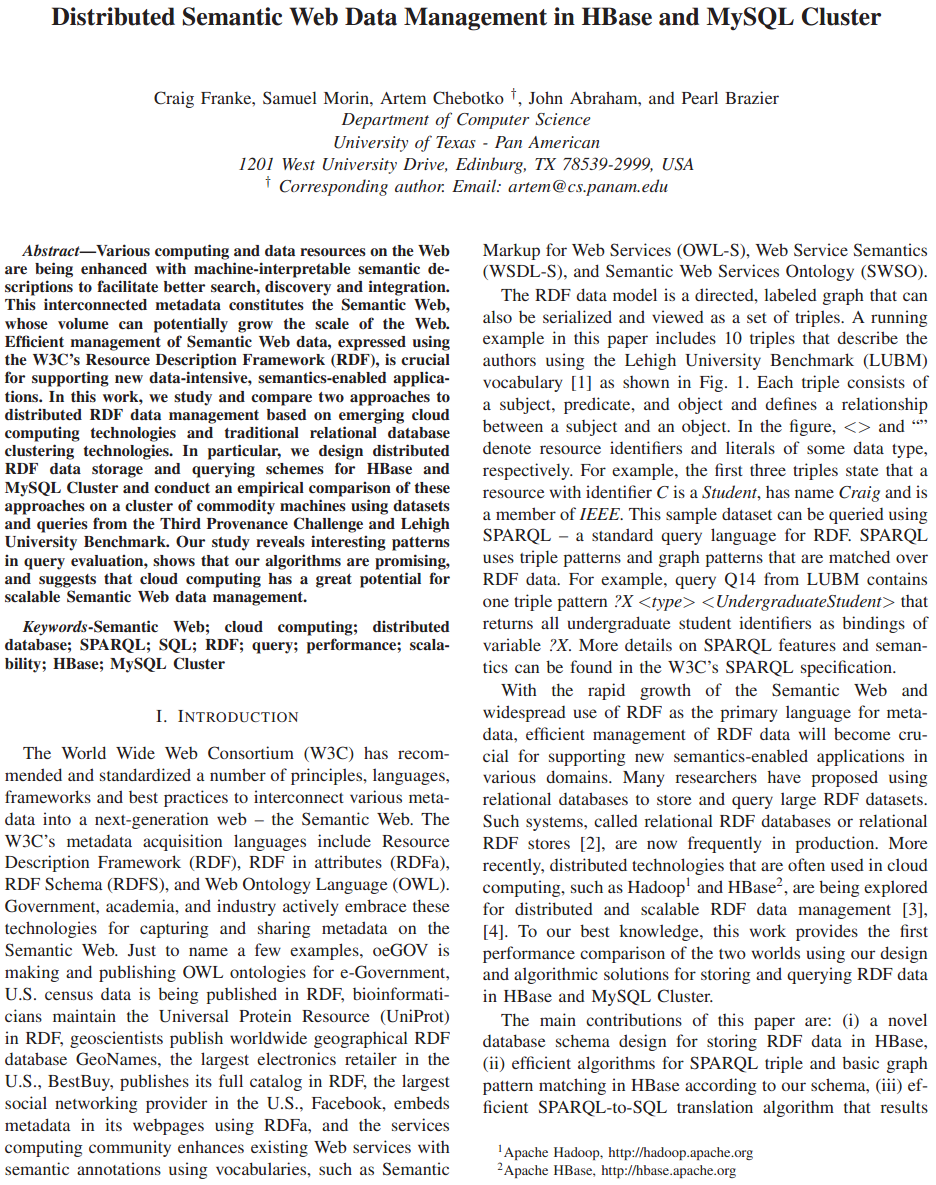
\includegraphics[scale=0.67]{photo/yingyu1.png}
\end{figure} 

\begin{figure}[!ht]
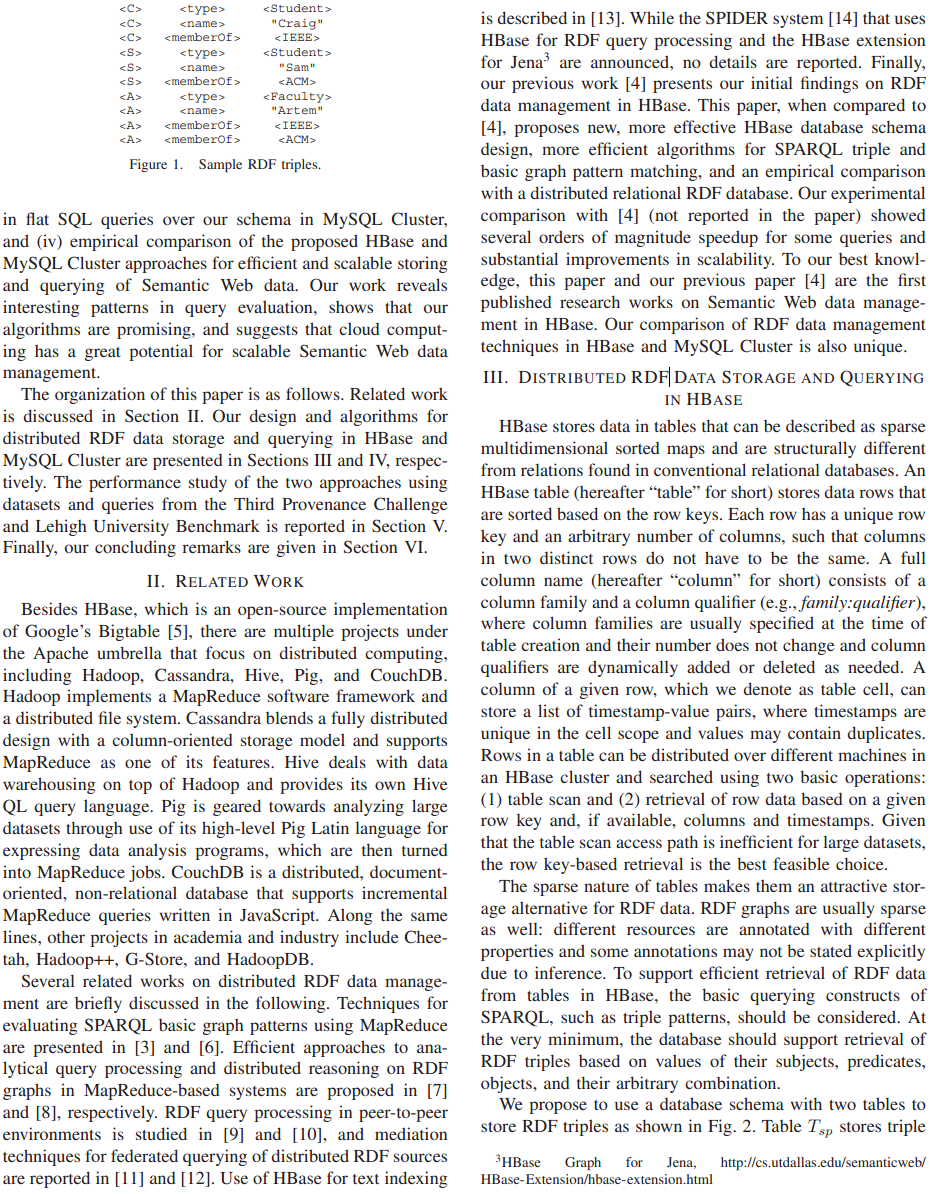
\includegraphics[scale=0.67]{photo/yingyu2.png}
\end{figure} 

\begin{figure}[!ht]
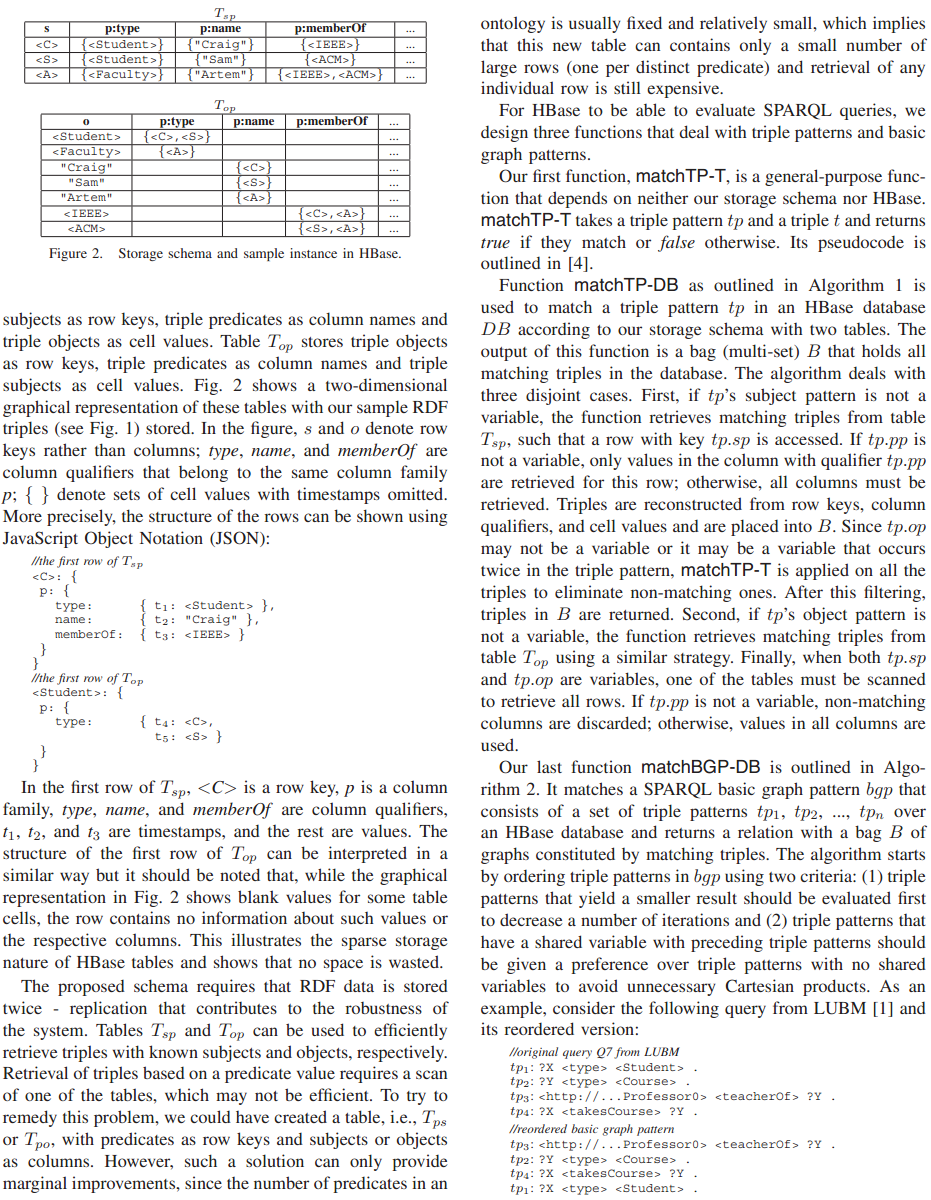
\includegraphics[scale=0.67]{photo/yingyu3.png}
\end{figure} 

\begin{figure}[!ht]
\includegraphics[scale=0.67]{photo/yingyu4.png}
\end{figure} 

\begin{figure}[!ht]
\includegraphics[scale=0.67]{photo/yingyu5.png}
\end{figure} 

\begin{figure}[!ht]
\includegraphics[scale=0.67]{photo/yingyu6.png}
\end{figure} 

\begin{figure}[!ht]
\includegraphics[scale=0.67]{photo/yingyu7.png}
\end{figure} 

\begin{figure}[!ht]
\includegraphics[scale=0.67]{photo/yingyu8.png}
\end{figure} 
\addcontentsline{toc}{chapter}{英文翻译}
\end{document}

